\documentclass[11pt]{article}

\usepackage[a4paper,margin=1in]{geometry}
\usepackage[T1]{fontenc}
\usepackage[utf8]{inputenc}
\usepackage{mathpazo}
\linespread{1.06}
\usepackage{amsmath,amssymb}
\usepackage{microtype}
\usepackage{booktabs,tabularx,threeparttable,array,multirow,longtable}
\usepackage{graphicx}
\usepackage[font=small,labelfont=bf,skip=6pt]{caption}
\usepackage{enumitem}
\usepackage[authoryear,round]{natbib}
\usepackage{xcolor}
\usepackage{tikz}
\usepackage{pgfplots}
\pgfplotsset{compat=1.16}
\definecolor{linkblue}{HTML}{1D5EA9}
\definecolor{ink}{HTML}{2B2B2B}
\definecolor{warm}{HTML}{E8672F}
\definecolor{grey}{HTML}{BDBAB0}
\usepackage[colorlinks=true,linkcolor=linkblue,citecolor=linkblue,urlcolor=linkblue,pdftitle={Predictability Without Monetization: A Point-in-Time Audit of Order-Flow Signals on the Moscow Exchange},pdfauthor={Oleg Sidorkin}]{hyperref}
\usepackage{url}

\setlist{itemsep=2pt,topsep=4pt}
\setlength{\parskip}{0pt}
\renewcommand{\arraystretch}{1.12}
\newcolumntype{L}{>{\raggedright\arraybackslash}X}
\newcolumntype{R}[1]{>{\raggedright\arraybackslash}p{#1}}
\newcommand{\pp}{\,pp}
\newcommand{\bp}{\,bp}

\title{\textbf{Predictability Without Monetization:\\
A Point-in-Time Audit of Order-Flow Signals\\
on the Moscow Exchange}}

\author{Oleg Sidorkin\\[3pt]\small Independent researcher\\[1pt]\small\texttt{osidorkin85@gmail.com}\thanks{Code, pre-registration plans, run logs and the hashes of the frozen forward-test models are public at \url{https://github.com/alterfo/moex-trader}, Apache License 2.0; the state of the repository used for this version is recorded in Appendix~\ref{app:checklist}. This paper is not investment advice. All errors are the author's.}}

\date{10 November 2026 \quad (version 5)\\[4pt]\small Preprint --- not peer reviewed; comments welcome}

\begin{document}
\maketitle

\begin{abstract}
\noindent
Does commercially available order-flow data predict the cross-section of Russian equity returns, and does the prediction survive realistic trading frictions? We audit this question for the 100 most liquid Moscow Exchange stocks, using five-minute order-book, order and trade statistics from the exchange's AlgoPack data, under a protocol that fixes hypotheses and thresholds before outcomes are read, builds the universe point-in-time, purges overlapping labels, and benchmarks results against permutation placebos and mechanism-free controls. A provenance rule is central: the exchange regenerated its 2020--2024 history, so records written more than 30 days after the trade date are excluded from every verdict; effects estimated on regenerated rows are about twice their real-time size. On the real-time window (January 2025--October 2026, 457 trading days), a regularized composite of 75 order-flow features forecasts 10-day abnormal returns with a mean daily rank IC of 0.096 (Newey--West $t=5.87$), 0.037 above a single-feature baseline, positive in seven of the eight calendar quarters, with placebos at zero. The prediction does not separate from price history. A 12-month momentum rank, which the composite does not contain, reaches IC 0.107 ($t=3.95$) on the same window; a momentum book nets at least as much as the composite book; the composite minus momentum contrast is $+0.019$\% per day with an interval that contains zero; and the 91\% of the composite's ranking power that is orthogonal to momentum converts into no separable net return. Monetization rests on measured inputs and still fails. The borrow fee is no longer assumed: across the 72 admitted names that resolve at the broker it ranges from 20.0\% to 125.0\% a year, median 25.0\%, quartiles 22.0\% and 36.9\%, with no name at the 17\% previously used as the base. At the measured median the book earns 0.038\% per day with a 95\% interval that includes zero, at 30\% 0.020\%, and it turns negative at the upper quartile. Borrow availability by date remains unmeasured, as do fills beyond the quoted spread. The declared forward rule has 15\% power against the observed effect: sixty dates can falsify the signal but cannot confirm it. Of 42 research directions run under the protocol, 33 failed their pre-specified criteria, four passed without beating the policy rate, and five remain leads awaiting frozen forward tests. We report the full ledger, the pitfalls that changed results, and the frozen forward tests.

\medskip
\noindent\textbf{Keywords:} order flow; limit order book; return predictability; transaction costs; short-sale costs; backtest overfitting; data provenance; Moscow Exchange.

\noindent\textbf{JEL:} G12, G14, C12, C52, C58.
\end{abstract}

\newpage

\section{Introduction}\label{sec:intro}

A forecasting signal and a trading strategy are different objects. The first is a statement about conditional expectations; the second must also survive the bid--ask spread, the cost and availability of short positions, execution delay, and the selection effects that accompany any search over many specifications. A large literature documents how often the second test fails where the first succeeds. Anomaly returns shrink after realistic trading costs \citep{novymarx2016}, concentrate in the short leg and largely vanish once borrow fees are charged \citep{muravyev2025}, decay after publication \citep{mclean2016}, and are frequently false discoveries once the number of tried specifications is taken into account \citep{harvey2016,harvey2020,chordia2020,hou2020}. Backtests are fragile because the researcher chooses among many variants on the same data \citep{bailey2014notices,bailey2017pbo,novymarx2015}, and because small violations of the decision-time information set inflate measured performance \citep{kaufman2012,zhang2026}.

Order flow is a natural place to look for predictability that is real. Microstructure theory links signed order flow to subsequent price changes \citep{kyle1985}. Empirically, order imbalance predicts returns of individual stocks and of the market at short horizons \citep{chordia2002,chordia2004}; order-flow imbalance across book levels explains contemporaneous price moves within and across stocks \citep{cont2014,cont2023}; and learned summaries of the limit order book carry forecastable information at several horizons \citep{kolm2023}. The same literature hints at why such signals can be hard to monetize: much of the predictability sits at horizons where turnover is large relative to the forecastable move.

This paper is an audit of what survives when both questions, prediction and monetization, are asked of one commercially available dataset under a protocol designed to prevent self-deception. The setting is the Moscow Exchange (MOEX) in 2025--2026. Following the restrictions on non-resident trading introduced in 2022, the market has been dominated by domestic retail investors, who accounted for 70.7\% of equity transactions in 2025 \citep{moex2026retail}. The Bank of Russia key rate ranged between 21\% and 14\% over our sample \citep{cbr2026}, so capital committed to a strategy has a high opportunity cost. Short selling is costly and patchy: only 10 of the 60 less-liquid stocks we checked were available to borrow at the broker. The exchange sells an order-flow dataset, AlgoPack, with five-minute ``super-candle'' statistics on trades, orders and the order book \citep{moexalgo}. As with the exchange analytics product that \citet{akyildirim2021} study for Borsa Istanbul, the practical question is whether a dataset any subscriber can buy contains cross-sectional information about future returns, and whether a subscriber can turn that information into net profit.

A data-provenance problem shapes the answer. AlgoPack's pre-2025 history was regenerated by the exchange after the fact. Every record carries a system timestamp (\texttt{SYSTIME}), and for equities, records written within 30 days of the trade date begin only on 3 January 2025. We use 2020--2024 only for specification and sign checks and issue every verdict on real-time records. The rule is consequential: the effect of the most predictive single feature is about twice as large on the regenerated history as in real time, every quantity we tuned on the regenerated history was more optimistic than its real-time counterpart, and an apparent improvement of a price-based classifier from order-flow inputs turned out to be market timing that disappears once features are demeaned within date.

We find four things. First, a regularized linear composite of 75 daily order-flow features forecasts the cross-section of 10-day abnormal returns on the real-time window with a mean daily rank information coefficient (IC) of 0.0957 (Newey--West $t=5.87$). It exceeds a baseline built on the 10-level book imbalance by 0.037, its permutation placebos sit at zero, its IC is positive in seven of the eight calendar quarters, and it retains 84\% of its IC when the forecast is one day stale. The ranking does not separate from price history. A 12-month momentum rank, which is not among the composite's inputs, reaches IC 0.1072 ($t=3.95$) on the same window and is confirmed on independent 2021--2024 prices (IC 0.038, $t=2.56$); run through the same book it nets at least as much as the composite; the pre-specified contrast between the two books is $+0.019$\% per day with an interval that contains zero; and the 91\% of the composite's ranking power that survives the removal of the momentum span does not convert into a separable net return. What the evidence establishes at the level of ranking is narrower than what it showed a month ago: the composite is not a momentum proxy, but neither is it worth more than one.

Second, monetization is not established, and the input that decides it is no longer assumed. The short-borrow terms of the admitted universe are now measured at the broker: across the 72 names that resolve, the annual rate runs from 20.0\% to 125.0\%, median 25.0\%, quartiles 22.0\% and 36.9\%, and no admitted name is available at the 17\% that the earlier draft used as its base. Carry enters the net return linearly at about 0.0037\pp\ per day per percentage point, so the whole curve follows from one run: the quoted-spread book earns 0.0679\% per day at 17\%, 0.0383\% at the measured median of 25\% ($t=0.89$, interval $[-0.040,+0.122]$), 0.0199\% at 30\%, and $-0.006$\% at the upper quartile. Under the flat 0.15\% per-side tariff of the live account the same book nets 0.0298\% at 17\% and nothing at 25\%. The headline of the previous draft, 0.075\% per day, was computed at the lowest rate in the programme's assumptions; it is an upper bound, not an estimate. The rest of the earlier reading stands: a one-day signal delay cuts the net return by 70\%, a two-day delay turns it negative, and the deflated Sharpe probability \citep{bailey2014dsr} is 0.685 after ten trials and 0.346 after one hundred. The tradable part of the signal decays much faster than its IC.

Third, part of the economics is now measured, part is still assumed, and the mapping remains one choice among many. The fee is measured, availability by date is not, and neither are executions beyond the quoted touch; we separate measured, bounded and assumed inputs explicitly (Section~\ref{sec:uncertainty}). Under the observed variance, detecting a true net return of 0.075\% per day with conventional power would take roughly 1,230 trading days, and demonstrating that the net return is smaller than the policy rate would take about 2,200; the sample cannot settle the economic question in either direction.

Fourth, the composite is one of 42 research directions run under the same protocol. Thirty-three failed their pre-specified criteria, four passed their criteria without earning more than the policy rate, and five remain leads awaiting frozen forward tests. The testing machinery appears calibrated: none of the mechanism-free control variables (lunar phase, planetary positions, geomagnetic activity, calendar-day parity, bitcoin volatility) or permutation placebos passed in the families for which we report them, and in the two largest libraries the number of nominal $p<0.05$ results was at or below the number expected by chance.

The paper's contributions are correspondingly modest and specific. It provides real-time, out-of-sample evidence on order-flow predictability in an emerging, retail-dominated market under a protocol fixed before outcomes were read. It documents and quantifies a provenance hazard in a widely available commercial dataset. It decomposes where the monetization of a real signal is lost and states which economic inputs would have to be measured to settle the question. And it reports a complete ledger of negative results and the pitfalls that changed results, in the spirit of recent reporting standards for forecasting and trading claims \citep{khushi2026}. It does not claim a trading strategy.

Section~\ref{sec:lit} relates the paper to the literature. Section~\ref{sec:data} describes the data, Section~\ref{sec:method} the protocol and methods. Section~\ref{sec:signal} reports the forecasting results and Section~\ref{sec:money} the monetization results. Section~\ref{sec:uncertainty} discusses economic uncertainty and pre-specified extensions, Section~\ref{sec:secondary} summarizes secondary results and leads, Section~\ref{sec:discussion} discusses implications, Section~\ref{sec:limits} lists limitations and Section~\ref{sec:conclusion} concludes. Appendices contain the feature definitions, secondary modules in detail, the ledger of all 42 directions, the catalogue of pitfalls, the calibration of the testing machinery, the frozen forward tests and a reproducibility checklist.

\section{Related literature}\label{sec:lit}

\paragraph{Order imbalance and order-book predictability.}
\citet{chordia2002} show that aggregate order imbalance predicts market returns, and \citet{chordia2004} that stock-level imbalance predicts next-day individual returns, with the effect reversing at longer lags. \citet{cont2014} relate price changes to order-flow imbalance at the best quotes, and \citet{cont2023} extend this to multiple book levels and cross-impact. \citet{kolm2023} find that deep networks fed with stationary order-flow inputs forecast returns at multiple short horizons. \citet{bogousslavsky2023} show that the volatility of order imbalance drives liquidity and is priced in the cross-section. \citet{akyildirim2021} show that order-imbalance analytics sold by Borsa Istanbul predict intraday excess returns. Our features also draw on measures of price impact \citep{kyle1985}, illiquidity \citep{amihud2002}, flow toxicity \citep{easley2012}, range-based volatility \citep{parkinson1980} and realized skewness \citep{amaya2015}; see \citet{bouchaud2018} for a synthesis. We differ in horizon (ten trading days rather than seconds to one day), in cross-sectional evaluation, and in our focus on whether a subscriber facing realistic frictions can monetize the signal.

\paragraph{From anomaly returns to net returns.}
\citet{novymarx2016} show that trading costs eliminate many anomalies, especially high-turnover ones, and that buy/hold spreads mitigate costs. \citet{garleanu2013} show that optimal trading with predictable returns and quadratic costs moves partially toward a target portfolio, which motivates our partial-adjustment books. \citet{muravyev2025} find that the average long--short anomaly return comes from the short leg and falls to roughly zero once borrow fees are charged. \citet{jacobs1998} and \citet{grinold2000b} show that the relative size of long and short exposures is a design choice with first-order consequences, a point we return to in Section~\ref{sec:mapping}.

\paragraph{Overfitting, multiple testing, leakage and long horizons.}
The deflated Sharpe ratio \citep{bailey2014dsr}, the probability of backtest overfitting \citep{bailey2017pbo}, minimum track-record length \citep{bailey2012sharpe} and the statistics of Sharpe ratios \citep{lo2002} address selection among backtests. Reality-check and step-wise procedures \citep{sullivan1999,white2000,hansen2005,romano2005}, false-discovery control \citep{benjamini1995,benjamini2001} and recent work on thresholds and replication \citep{harvey2016,harvey2020,chordia2020,hou2020,giglio2021} address multiplicity; \citet{novymarx2015} shows that combining several signals chosen in-sample inflates $t$-statistics far beyond conventional levels. Purging and embargoing overlapping labels follow \citet{lopezdeprado2018}; \citet{kaufman2012} formalize leakage, and \citet{zhang2026} show that single protocol deviations can manufacture apparent alpha. Overlapping long-horizon outcomes reduce the effective sample and can make conventional standard errors over-confident \citep{hjalmarsson2011,boudoukh2019}. Our protocol borrows from pre-registration \citep{nosek2018} and equivalence testing \citep{lakens2017,lakens2018}, and our reporting follows the checklist logic of \citet{khushi2026}.

\paragraph{Machine learning and foundation models.}
\citet{gu2020} document gains from machine learning in cross-sectional return prediction. Evidence for pretrained time-series foundation models is mixed: \citet{rahimikia2025} and \citet{alonso2026} find small or inconsistent gains for off-the-shelf models such as TimesFM \citep{das2024}. We report a negative transfer result consistent with that evidence.

\paragraph{The Russian equity market.}
Studies of the Russian market have focused on sanctions \citep{ankudinov2017,dovbnya2020} and, recently, news sentiment \citep{makeeva2026}, which finds sentiment to be mainly a reactive indicator. We are not aware of published work on the cross-sectional content of AlgoPack order-flow data or of real-time evaluations that account for its regenerated history. One of our portfolio modules replicates the higher-moment VAR-ICA-MGARCH approach of \citet{mikhaylov2026}; see also \citet{lassance2022}.

\section{Data and sample construction}\label{sec:data}

\subsection{Sources}

Table~\ref{tab:data} lists the data. All sources are public or available by exchange subscription; no proprietary or internal data are used. The core dataset is AlgoPack \citep{moexalgo}: for every instrument and five-minute bar, four ``super-candle'' sets. \texttt{tradestats} summarizes trades, including buyer- and seller-initiated value, volume and counts and side-specific VWAPs. \texttt{obstats} summarizes the order book: best-quote spread, the spread over 10 levels and for a RUB~1 million order, the number of levels, resting value and volume on each side, and normalized imbalances $(\text{bid}-\text{ask})/(\text{bid}+\text{ask})$ at the best quotes and over 10 levels. \texttt{orderstats} summarizes order placements and cancellations by side. \texttt{hi2} reports end-of-day participant-concentration indices. For equities the archive covers 1,775 trading days from 3 January 2020, about 250 stocks per day including later-delisted names, and 146 million rows across the three intraday sets.

\begin{table}[htbp]
\centering
\begin{threeparttable}
\caption{Data sources}\label{tab:data}
\small
\begin{tabularx}{\textwidth}{@{}R{3.3cm}LR{4.2cm}@{}}
\toprule
Source & Content & Coverage \\
\midrule
MOEX ISS (open API) & Daily equity candles (open, close, turnover); IMOEX, RVI, RTSI and sector indices; government-bond indices; USD/RUB; 10-minute equity candles & 2014--2026; 719 stocks ever traded on the main board (TQBR), incl.\ delisted; 881,385 stock-days \\
MOEX AlgoPack (subscription) & Five-minute \texttt{tradestats}, \texttt{obstats}, \texttt{orderstats}, \texttt{hi2} for equities, futures and FX & From 2020-01-03; equities 1,775 days, $\approx$250 stocks/day, 146 mn rows \\
Broker dividend calendar & Last buy date and net dividend per share & 2,152 records (broad panel); 115 events for the top 100, 2021--2026 \\
News archive & Ticker-tagged headlines with time stamp, source and source-trust weight & 155,601 headlines, 2022-01 to 2026-10 \\
Macro and external series & Policy rate, CNY/RUB, USD/RUB, Brent, gold in RUB, ETF turnover, commodities, weather, GDELT tone, geomagnetic Kp index, bitcoin (control only) & Daily, from 2019 where available \\
\bottomrule
\end{tabularx}
\begin{tablenotes}\footnotesize
\item Notes: Sources used only in secondary modules (retail open interest in futures, S\&P~500 history for calendar tests, a public Russian financial-news corpus for classifier training) appear in Appendix~\ref{app:secondary}.
\end{tablenotes}
\end{threeparttable}
\end{table}

\subsection{Data provenance and the real-time rule}\label{sec:provenance}

Each AlgoPack row carries a field \texttt{SYSTIME} recording when the row was written. A row whose \texttt{SYSTIME} is more than 30 days after its trade date was not written in real time; we call it \emph{regenerated}. For equities, real-time rows start on 3 January 2025. For futures, \texttt{tradestats} and \texttt{obstats} become real-time in May 2025 and \texttt{orderstats} in August 2026; FX sets switch at different dates in 2025 and 2026.

We adopt one rule for the whole program. Rows with $\texttt{SYSTIME} > \text{trade date} + 30$ days may be used for fitting, specification and sign checks, but never for a verdict. Verdicts use only real-time rows. Section~\ref{sec:regen} quantifies what the rule changes. Regenerated rows are not necessarily wrong; the point is that we cannot verify that they reflect information available at the time, and that their statistical properties differ from real-time rows.

\subsection{Prices, calendar and corporate actions}

A trading day is a day on which at least 30 stocks are quoted. MOEX trades equities on some Saturdays while the IMOEX index is not computed on weekends, so a 10-bar window spans on average 9.31 panel bars, 9.31 trading days counted on the MOEX equity calendar (Saturdays excluded) and 12--13 calendar days; all windows are defined in panel bars, and the three counts are stated separately because they are not interchangeable. The market closure of 25 February to 28 March 2022 is excluded: any return with either end point inside it is dropped.

The daily close is the \texttt{pr\_close} of the last five-minute bar of the main session, whose bar-end labels run from 10:05 to 18:50; morning and evening sessions are excluded. A one-day price change below $-45\%$ or above $+80\%$ is treated as a split or consolidation and dropped. AlgoPack prices are unadjusted and ISS prices are on a different scale for some stocks, so the two sources are never mixed within one return. Ticker renames (YNDX$\to$YDEX, TCSG$\to$T) are mapped to one identifier; without this, up to 70\% of rows for the affected stocks are lost.

The ex-dividend date is the first trading day after the last buy date. In all order-flow studies, the ex-date and the trading days immediately before and after it are excluded for that stock: its return, its feature row and any outcome window containing it.

An intraday bar enters a feature only if it is present in all three intraday sets, and a daily feature requires at least 20 such bars before 18:30. Days with fewer than 80\% of the stock's median annual bar count are dropped. Before any outcome was read, we checked file counts against the ISS calendar, the share of zero-value bars and the agreement of the AlgoPack close with ISS (median absolute deviation 0.18--0.33\% for stocks unaffected by splits). A year in which more than 2\% of stock-days failed these checks would have been dropped rather than repaired.

\subsection{Universe and returns}

The main universe is the point-in-time top 100: on each date $d$, the 100 stocks with the highest median daily turnover over the previous 60 trading days (at least 40 observations). Membership is recomputed daily and uses only information before $d$. A ``thin'' universe consists of ranks 101--400 on the same ranking. With $C_{i,d}$ the close of stock $i$ on day $d$ and $U_d$ the universe on $d$,
\begin{align}
r_{i,d} &= \ln\!\left(C_{i,d}/C_{i,d-1}\right), & ab_{i,d} &= r_{i,d}-\frac{1}{|U_d|}\sum_{j\in U_d} r_{j,d},\\
y^{(h)}_{i,d} &= \ln\!\left(\frac{C_{i,d+h}}{C_{i,d}}\right)-\frac{1}{|U_d|}\sum_{j\in U_d}\ln\!\left(\frac{C_{j,d+h}}{C_{j,d}}\right), \label{eq:y}
\end{align}
so $y^{(h)}_{i,d}$ is the $h$-day abnormal return from the close of $d$. The main horizon is $h=10$.

\subsection{Timing of signals and execution}\label{sec:timing}

Features use bars ending no later than 18:30. Orders submitted at 18:30 can still participate in the closing auction, which accepts orders until 18:50, so a position taken at the close of day $d$ on a signal computed at 18:30 is feasible. Columns that depend on bars after 18:30 (full-session turnover, closing-auction imbalance) are excluded from the composite. Including them would have changed the composite IC by only 0.00003, but they are not available at the decision time.

\subsection{Sample design}\label{sec:design}

Figure~\ref{fig:design} summarizes the design. The composite panel has 163,709 stock-days on 1,644 dates from January 2020 to 20 October 2026. Hyper-parameters are chosen on the regenerated fitting sample from July 2022 to December 2024. The verdict window runs from 3 January 2025 to 16 October 2026 (457 trading days for the main book) and is split into halves at 5 January 2026. The book and the IC series do not have the same length, and the difference is mechanical: a daily IC needs a matured 10-day outcome, so with the data cut of 20 October 2026 the last seven dates have no outcome yet and the IC series stops at 450 dates, while the book, which marks positions to market, runs to 457. A frozen forward test began on 22 October 2026.

\begin{figure}[htbp]
\centering
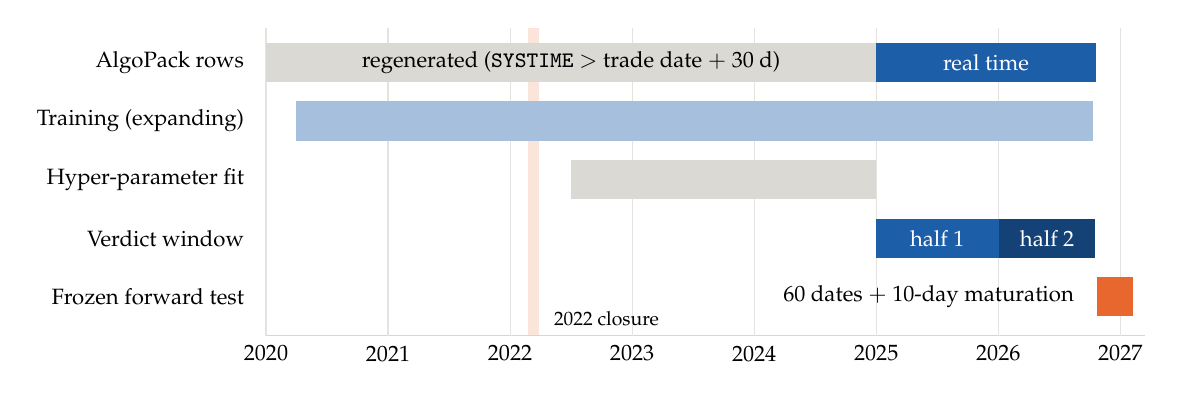
\begin{tikzpicture}[x=1.55cm,y=0.62cm,font=\footnotesize]
\fill[warm!18] (2.15,-0.6) rectangle (2.24,5.7);
\draw[grey!60] (0,-0.6) -- (7.2,-0.6);
\foreach \yr in {2020,...,2027}{
  \pgfmathsetmacro{\xx}{\yr-2020}
  \draw[grey!40] (\xx,-0.6) -- (\xx,5.7);
  \node[below] at (\xx,-0.6) {\yr};
}
\node[left] at (-0.1,5) {AlgoPack rows};
\fill[grey!55] (0,4.6) rectangle (5.0,5.4);
\fill[linkblue] (5.0,4.6) rectangle (6.8,5.4);
\node at (2.5,5) {regenerated (\texttt{SYSTIME} $>$ trade date $+$ 30 d)};
\node[white] at (5.9,5) {real time};
\node[left] at (-0.1,3.8) {Training (expanding)};
\fill[linkblue!40] (0.25,3.4) rectangle (6.78,4.2);
\node[left] at (-0.1,2.6) {Hyper-parameter fit};
\fill[grey!55] (2.5,2.2) rectangle (5.0,3.0);
\node[left] at (-0.1,1.4) {Verdict window};
\fill[linkblue] (5.0,1.0) rectangle (6.01,1.8);
\fill[linkblue!70!black] (6.01,1.0) rectangle (6.79,1.8);
\node[white] at (5.5,1.4) {half 1};
\node[white] at (6.4,1.4) {half 2};
\node[left] at (-0.1,0.2) {Frozen forward test};
\fill[warm] (6.81,-0.2) rectangle (7.1,0.6);
\node[anchor=east] at (6.7,0.2) {60 dates $+$ 10-day maturation};
\node[anchor=west,font=\scriptsize] at (2.28,-0.25) {2022 closure};
\end{tikzpicture}
\caption{Sample design. AlgoPack equity rows before 2025 were regenerated after the fact and are used only for fitting and sign checks. Models are trained on an expanding window with an 11-trading-day embargo before each quarterly test block. Verdicts are read once on the real-time window, split into halves at 5 January 2026. The forward test is read once after 60 new dates and 10-day outcome maturation.}\label{fig:design}
\end{figure}


\section{Protocol and methods}\label{sec:method}

\subsection{Pre-specification and decision rules}\label{sec:protocol}

The protocol is designed so that the researcher cannot adapt criteria to results. Its rules are:
\begin{enumerate}[label=(\roman*)]
\item \emph{Plan before outcomes.} Each study has a written plan with feature definitions, the expected sign, windows, controls, family size, thresholds, the economic criterion and the requirement that the sign hold in both halves. The plan is time-stamped before any outcome is computed.
\item \emph{One read.} A verdict window is ``spent'' by one test. If a window has already been viewed for another question, the plan says so and any positive result is labelled a lead, not a finding.
\item \emph{Two statuses.} Confirmatory rows have hard thresholds and verdicts. Exploratory rows are screened by the \citet{benjamini1995} procedure at $q=0.10$ and can only become \emph{leads}. A lead becomes confirmatory only through a new plan that copies its definition verbatim.
\item \emph{Failure is final.} A failure closes the direction for the same definitions. Changing windows, signs or controls after seeing results requires a new plan with a new family size.
\item \emph{Mechanism controls.} Each series runs alongside permutation placebos and mechanism-free controls (lunar phase, Saturn's longitude, the geomagnetic Kp index, Mercury retrograde, calendar-day parity, bitcoin volatility). A hit by any control invalidates all hits of the same series.
\item \emph{Independent pre-run review.} Before each run the code and plan were read by a second reviewer, a separate large-language-model instance with read-only access, tasked with finding look-ahead leakage, plan--code mismatches and unattainable thresholds. Its findings were recorded as amendments before the run; amendments made after the first look at numbers are recorded separately and flagged.
\item \emph{Frozen forward tests.} A lead is frozen: fitted models are saved with their SHA-256 hashes, together with the portfolio rule and thresholds. It is read once after a pre-set number of new dates and never extended or restarted.
\item \emph{Power on record.} Before each run the plan states the smallest detectable effect. For the composite, the Newey--West standard error of the IC increment over 450 dates is 0.0147, so an increment of 0.063 is needed for $|t|=3.45$ at 80\% power; the earlier draft printed 0.07 from the level IC standard error, and the difference is corrected here. The same rule was not applied to the confirmation rule itself, which is the defect repaired in Section~\ref{sec:uncertainty}.
\item \emph{Full count.} A registry of all attempts is kept, because the number of trials enters the deflated Sharpe ratio.
\end{enumerate}
Plans were time-stamped by the commit history of the public repository, not by an external registry. We return to this limitation in Section~\ref{sec:limits}.

\subsection{Features}

\paragraph{Five base features.} With sums over the joint bars of day $d$ up to 18:30 and $v^b,v^s$ the buyer- and seller-initiated traded value,
\begin{align}
A1&=\frac{\sum (v^b-v^s)}{\sum v}, & A2&=\frac{\sum \mathrm{imb}^{(10)}_{\mathrm{val}}\,v}{\sum v}, & A3&=\overline{\mathrm{imb}^{\mathrm{bbo}}_{\mathrm{val}}},\\
A4&=\frac{(P^b-X^b)-(P^s-X^s)}{P^b+P^s}, & A5&=\frac{\sum X}{\sum P},
\end{align}
where $\mathrm{imb}^{(10)}_{\mathrm{val}}$ is the value imbalance over 10 book levels, $\mathrm{imb}^{\mathrm{bbo}}_{\mathrm{val}}$ the imbalance at the best quotes, and $P$ and  value of placed and cancelled orders by side. The denominator of A4 counts placed orders only, so the statistic is net flow per unit of gross placement rather than per unit of net activity; the choice is stated because the written form does not make it obvious. A1 is trade imbalance, A2 book imbalance, A3 imbalance at the touch, A4 net order flow and A5 cancellation intensity. Signs were fixed in advance as ``more buyers, higher return'' except for A5, which is tested two-sided.

\paragraph{The 75-feature composite.} Table~\ref{tab:families} groups the composite's inputs; Appendix~\ref{app:features} defines each. The families cover imbalances (including intraday sub-windows and within-stock ``surprise'' $z$-scores), book shape and depth, spreads, trade size and activity, aggressor prices, order placement and cancellation, realized volatility and jumps, and eight microstructure measures. One feature, \texttt{ThinBid}, turned out to be identically zero by construction (Appendix~\ref{app:pitfalls}); we keep it in the count for transparency. Three controls, the within-date ranks of the past 1-, 5- and 20-day returns, are always included so that the composite must add to short-term reversal and one-month momentum. Longer-horizon momentum is \emph{not} among the inputs; Section~\ref{sec:momentum} shows why this matters.

Inputs were included by feature family and by decision-time availability, not by their individual performance. Each is ranked within date across stocks that have it (at least 30) and scaled to $[-0.5,0.5]$ as $(\mathrm{rank}-1)/(n-1)-0.5$; missing values are set to 0, the neutral rank.

\begin{table}[htbp]
\centering
\caption{Feature families in the composite}\label{tab:families}
\small
\begin{tabularx}{\textwidth}{@{}R{3.1cm}L@{}}
\toprule
Family & Content \\
\midrule
Order and trade imbalance & A1, A2, A3, volume-based book imbalance; A2 in early, late and half-session windows; within-stock ``surprise'' $z$-scores of A1 and A2; dispersion of bar-level imbalance; slope of cumulative imbalance \\
Book shape & Average depth (resting value on both sides); level asymmetry; open-to-close depth ratio; number of joint bars \\
Spreads & Mean best-quote, 10-level and RUB 1 mn spreads; their ratios, dispersion and last value; morning compression; spread over bar price volatility \\
Trade size and activity & Mean, median and dispersion of trade size; buyer and seller ticket size; trade count and its imbalance; top-3 bar concentration; share of idle bars; Amihud illiquidity \\
Aggressor prices & Buyer--seller VWAP gap; close location in the day's range; deviation of close from VWAP; last-hour and morning returns; intraday profile shares \\
Orders & Net order flow A4 (full day, open, close windows); cancellation intensity A5; cancellation asymmetry; placement aggressiveness; order size asymmetry; orders placed relative to traded value and to book depth \\
Volatility and jumps & Realized volatility of five-minute closes; up and down semivariances; maximum jump; Parkinson range ratio; mean bar price volatility \\
Microstructure & VPIN-like ratio; Kyle-lambda slope; flow--return correlation; flow and book-imbalance autocorrelations; realized skewness; turnover tilt \\
Controls (always in) & Within-date ranks of past 1-, 5- and 20-day returns \\
\bottomrule
\end{tabularx}
\end{table}

\subsection{The composite model}\label{sec:model}

Let $x_{i,d}\in\mathbb{R}^{78}$ be the scaled inputs, centred within date, and $y_{i,d}$ the within-date rank of $y^{(10)}_{i,d}$ scaled to $[-0.5,0.5]$. With $X$ and $y$ stacked over the training rows ($n$ observations, no intercept), the ridge component \citep{hoerl1970} is
\begin{equation}
\hat\beta_{\mathrm R}=\left(X^\top X/n+\lambda_{\mathrm R}I\right)^{-1}X^\top y/n,\qquad \lambda_{\mathrm R}=0.003,
\end{equation}
and the elastic-net component \citep{zou2005} solves
\begin{equation}
\min_\beta\ \frac{1}{2n}\|y-X\beta\|_2^2+\lambda_{\mathrm{EN}}\Big[\alpha\|\beta\|_1+\tfrac{1-\alpha}{2}\|\beta\|_2^2\Big],\qquad \alpha=0.5,\ \lambda_{\mathrm{EN}}=0.001,
\end{equation}
by coordinate descent \citep{friedman2010} (at most 500 passes, tolerance $10^{-7}$). The composite forecast is the average of the two predictions. The baseline is a ridge regression ($\lambda=0.001$) on A2 and the three return controls only.

Hyper-parameters were chosen only on the fitting sample (July 2022 to December 2024); Section~\ref{sec:grids} reports the grids. Because order-flow effects are stronger on the regenerated fitting sample (Section~\ref{sec:regen}), the selection is optimistic by construction; the verdict is read once on the real-time window.

Estimation is walk-forward with an expanding window from April 2020. Each quarterly test block is predicted by a model trained only on dates at least 11 trading days before the block's start, which purges overlapping 10-day labels and adds a one-day embargo \citep{lopezdeprado2018}. The verdict window contains seven quarterly blocks.

\paragraph{Why the average and not the better component.} On the verdict window the ridge component has IC 0.0970, the elastic net 0.0915 and their average 0.0957, so the average is 0.0013 below the better component. That gap is not a reason to reselect: the two components tie on the fitting sample (0.1328 for ridge, 0.1326 for the elastic net), where the average was fixed in advance, and 0.0013 is a tenth of the standard error of the composite IC over the same window, i.e. a difference well inside sampling noise. Choosing the component with the higher verdict-window IC after reading the verdict window would add one more trial to a family of 41 and would spend the protection the pre-registration buys. We report both components separately and keep the average, and we flag the gap here so that it is visible rather than buried in a table.

\subsection{Statistical inference}\label{sec:inference}

\paragraph{Information coefficient.} The daily IC is the Pearson correlation between within-date ranks of the forecast and of the outcome, i.e.\ a Spearman correlation. We report its mean over dates and a Newey--West $t$-statistic \citep{newey1987} with Bartlett weights and $L$ lags,
\begin{equation}
\hat V=\hat\gamma_0+2\sum_{l=1}^{L}\Big(1-\frac{l}{L+1}\Big)\hat\gamma_l,\qquad t=\bar x/\sqrt{\hat V/n},
\end{equation}
with $L=10$ for 10-day outcomes, $L=5$ for one-day outcomes and $\max(5,h)$ in general; where noted, $L$ is chosen by the \citet{andrews1991} AR(1) plug-in rule.

\paragraph{Overlapping horizons.} Daily 10-day outcomes overlap, so 457 daily ICs contain only about 46 non-overlapping 10-day periods. Newey--West with $L$ equal to the horizon and the block bootstrap with blocks at least as long as the horizon are designed for this dependence, but both can be over-confident when the effective sample is small \citep{hjalmarsson2011,boudoukh2019}. We therefore add tests that do not rely on a long-run variance estimate: sign tests across disjoint quarterly and monthly blocks (Section~\ref{sec:robust}), and the requirement that every verdict hold in both halves and show no significant opposite sign in either calendar year.

\paragraph{Fama--MacBeth regressions.} For single features we run daily cross-sectional regressions of the outcome rank on the feature rank and controls \citep{fama1973}: the returns of days $t,t-1,\dots,t-5$, log turnover relative to its 20-day mean, and the mean 10-level spread. A control is dropped if its mean rank correlation with the feature exceeds 0.7. When the outcome is realized within the same day, controls are lagged one day; otherwise the outcome leaks into the controls (Appendix~\ref{app:pitfalls}).

\paragraph{Halves.} Each result must have the same sign in both pre-specified halves. A verdict additionally fails if either calendar year 2025 or 2026 shows the opposite sign with $|t|\ge 2$.

\paragraph{Block bootstrap.} Daily series (IC, net returns) are resampled in blocks of consecutive dates \citep{kunsch1989}: block length 10 (or $\max(10,H)$ for horizon $H$), 5,000 resamples, percentile intervals. Seeds are fixed in the plans.

\paragraph{Placebos.} The main placebo permutes feature vectors across stocks within each date (five seeds). It preserves all date-level moments of the features and destroys the link between a stock and its features. If a placebo passes, the series of tests is void. Time-shift placebos (260, 380 or 520 dates) and, for binary state variables, circular shifts of at least 20 dates are also used; the circular-shift $p$-value is $(1+\#\{|D^*|\ge|D|\})/(1+\#\text{shifts})$.

\paragraph{Multiple testing.} For a family of $M$ features with eigenvalues $\lambda_k$ of their mean cross-sectional rank-correlation matrix, the effective number of tests is $M_{\mathrm{eff}}=1+(M-1)(1-\mathrm{Var}(\lambda)/M)$ \citep{nyholt2004}, computed before any outcome is read. The threshold is $|t|\ge\max\{3.0,z_{1-0.025/M_{\mathrm{eff}}}\}$ or $p\le 0.05/M_{\mathrm{eff}}$; the floor of 3.0 follows \citet{harvey2016}. Benjamini--Hochberg control at $q=0.05$ or $0.10$ is used where stated.

\paragraph{Deflated Sharpe ratio.} For a daily net-return series with Sharpe ratio $\widehat{SR}$, $T$ observations, skewness $\gamma_3$ and kurtosis $\gamma_4$,
\begin{equation}
\mathrm{PSR}(SR_0)=\Phi\!\left(\frac{(\widehat{SR}-SR_0)\sqrt{T-1}}{\sqrt{1-\gamma_3\widehat{SR}+\frac{\gamma_4-1}{4}\widehat{SR}^2}}\right),\label{eq:psr}
\end{equation}
and the deflated Sharpe ratio sets $SR_0$ to the expected maximum Sharpe ratio of $N$ independent skill-less trials, $SR_0=\sqrt{V}\big[(1-\gamma)\Phi^{-1}(1-1/N)+\gamma\Phi^{-1}(1-1/(Ne))\big]$ with $\gamma_{E}\approx0.5772$ and $V=1/T$ \citep{bailey2014dsr}. Because the effective number of trials is unknowable, we report $N\in\{1,10,50,100,300,800\}$. Because daily book returns are autocorrelated, we also report a variant in which $V$ is inflated by the series' autocorrelation factor. The probability of backtest overfitting, estimated by combinatorially symmetric cross-validation with $S=16$ \citep{bailey2017pbo}, enters the deployment gate of the price-based classifier.

\subsection{Portfolio construction and costs}\label{sec:portfolio}

On each date with at least 40 forecasts, stocks are sorted by forecast; the top and bottom quintiles form long and short legs. Within each leg, target weights are proportional to $1/\sigma_i$, the standard deviation of the stock's abnormal return over its last 20 observations, normalized to sum to one, so the book is dollar-neutral with gross exposure 2. Let $a_{i,d}$ be the target weight. The daily book holds $w_{i,d}=a_{i,d}$; the partial-adjustment book holds
\begin{equation}
w_{i,d}=(1-r)\,w_{i,d-1}+r\,a_{i,d},\qquad r\in\{1,0.5,0.33,0.2,0.1,0.05\},\label{eq:adj}
\end{equation}
in the spirit of \citet{garleanu2013}. The daily net return is
\begin{equation}
\mathrm{net}_d=\sum_i w_{i,d}\,f_{i,d+1}-\sum_i|w_{i,d}-w_{i,d-1}|\,c_{i,d}-\frac{b}{252}\sum_{w_{i,d}<0}|w_{i,d}|,\label{eq:net}
\end{equation}
where $f_{i,d+1}$ is the simple close-to-close return, $c_{i,d}$ the one-way cost and $b$ the annual borrow rate. The adjustment speed is chosen on the fitting sample: $r=0.33$ under flat costs and $r=0.5$ under quoted-spread costs.

Three cost models are used. \emph{Flat:} 0.15\% per side, the retail broker tariff. \emph{Quoted spread:} 0.05\% commission plus half the stock-day's best-quote spread (0.15\% if unavailable); half-spreads average about 1.8\bp for the most liquid third and 9--45\bp for thin stocks. \emph{RUB 1 mn order (stress):} 0.05\% plus half the spread for an order of about RUB 1 million. Borrow is charged at three annual rates: the measured median of the admitted universe, 25.0\%, as the base after the measurement of Section~\ref{sec:borrow}; 17\%, the secondary quote used in the earlier draft and now known to be below every measured name, kept only for comparability with the published tables; and 36.9\%, the measured upper quartile. Variants include a long-only book measured against the equal-weighted universe (no borrow), entry at the next open, and a sector-neutral forecast demeaned within five fixed sector groups.

\subsection{Verdict criteria for the composite}\label{sec:criteria}

The composite was evaluated once on the real-time window against three pre-specified criteria.
\begin{enumerate}[label=(\arabic*)]
\item \emph{Signal:} the mean daily out-of-fold IC of the composite minus that of the baseline is positive with a 95\% bootstrap interval above zero; positive in both halves; and the composite beats its placebo with an interval above zero in at least four of five seeds.
\item \emph{Economics:} the dollar-neutral book (flat costs, 25\% borrow as the measured median, 36.9\% as the upper-quartile stress) has a net mean with a 95\% interval above zero in both halves, and placebo books have non-positive means.
\item \emph{Execution:} the partial-adjustment book beats the daily book with an interval above zero.
\end{enumerate}
Passing (1) and (2) would make the composite a lead with a frozen forward rule. A later plan (Section~\ref{sec:book}) re-evaluated economics under quoted-spread costs with horizons $H\in\{10,20,40\}$ selected on the fitting sample, with the gate that the net mean's 95\% interval lie above zero, the mean be positive in both halves and the placebo books be non-positive.

\paragraph{One standard or two?} Criterion (1) is an interval test, while Section~\ref{sec:inference} applies $|t|\ge3.0$ to the single-feature families. The difference is deliberate but it is a difference, and the reader is entitled to see it stated rather than to infer it. The threshold prices the search over 28 and 94 candidate features; the composite's increment was not selected over that family, because its inputs were fixed by family and by decision-time availability before the window was touched and its weights are fitted out-of-fold, so the pre-registered gate for it is the interval of the increment. We nevertheless report the stricter reading next to the looser one, because the two do not agree: the increment over the baseline has $t=2.51$ and does not clear 3.0, while the momentum rank's own level IC has $t=3.95$ and does. A reader who applies one threshold to both statistics should conclude that the composite's ranking advantage over the baseline is the weaker of the two claims, and that is how we state it in the abstract and in Section~\ref{sec:signal}. Finally, rule (ii) of the protocol says that a positive result read on a window already used for another question is a lead, not a finding. The real-time window was used by the single-feature family before the composite was evaluated, so the composite's result is reported throughout as a lead, with the frozen forward test of Section~\ref{sec:extensions} as its only confirmation path.

\section{Results I: the signal}\label{sec:signal}

\subsection{Single features: strong statistics, marginal economics}

The first plan tested 12 hypotheses built mainly on the five base features (next-day abnormal returns, intraday windows, level-crossing events) plus one market-level concentration signal. Only A2, the 10-level book imbalance, passed: Fama--MacBeth $t=+19$ and a net return of 0.049\% per day for a long top-quintile book against the universe at 0.15\% per side, positive in both halves. A version hedged with an IMOEX short failed, with a negative second half. Before the hedge, the net return is 0.049\% per day, 12.3\% a year, without the controls and 0.023\% per day, 5.8\% a year, with them; the earlier draft quoted a 3--6\% range that does not follow from either number and is withdrawn. This plan's halves (January 2020 to June 2023, July 2023 to October 2026) predate the provenance rule and rely mostly on regenerated rows, so in retrospect we treat its result as exploratory.

The second plan tested 100 hypotheses on the real-time window (about 420 dates), with 28 confirmatory rows (effective family size 22.574; threshold $|t|\ge3.060$) and 72 exploratory rows. Each confirmatory row required both a Fama--MacBeth $t$ above threshold and a positive net return in both halves for a long top-quintile book. None of the 28 passed. The closest was weekly-rebalanced A2, with $t=+5.52$ but a first-half net return of $-0.003\%$ per day. Of 63 screened exploratory rows, 17 survived Benjamini--Hochberg at $q=0.10$, ten of them variants of A2. Single order-flow features are statistically strong and economically marginal, which motivates pooling them.

\subsection{The composite forecasts the cross-section}\label{sec:momentum}

Table~\ref{tab:signal} reports the verdict. The composite's mean daily IC on the real-time window is 0.0957 with a Newey--West $t$ of 5.87 and a bootstrap interval of $[0.0693,0.1294]$. The increment over the A2 baseline is 0.0368 with a 95\% interval of $[0.0147,0.0663]$, above zero and positive in both halves. Placebos trained on within-date permuted features stay at zero in all five seeds (IC between $-0.0042$ and $+0.0052$). The signal criterion is met.

\begin{table}[htbp]
\centering
\begin{threeparttable}
\caption{Signal verdict on the real-time window}\label{tab:signal}
\small
\begin{tabularx}{\textwidth}{@{}L r r@{}}
\toprule
 & Mean daily IC & NW $t$ \\
\midrule
Composite (75 order-flow features $+$ 3 controls) & 0.0957 & 5.87 \\
\quad 95\% block-bootstrap interval; halves & $[0.0693,\,0.1294]$; 0.0853 / 0.1092 & \\
Baseline (A2 $+$ 3 controls) & 0.0589 & \\
\quad 95\% block-bootstrap interval & $[0.0389,\,0.0778]$ & \\
Increment, composite minus baseline & 0.0368 & 2.51 \\
\quad 95\% block-bootstrap interval; halves & $[0.0147,\,0.0663]$; 0.0431 / 0.0286 & \\
Within-date permutation placebo, 5 seeds & $-0.0042$ to $+0.0052$ & \\
\addlinespace
\multicolumn{3}{@{}l}{\emph{Momentum comparison (E1, pre-specified after the window closed)}} \\
256-day momentum rank alone, same window\tnote{a} & 0.1072 & 3.95 \\
Composite residual after projection on the momentum rank\tnote{b} & 0.0869 & 7.33 \\
Composite plus 256- and 120-day momentum (descriptive) & 0.1062 & \\
\addlinespace
\multicolumn{3}{@{}l}{\emph{Variants (descriptive)}} \\
Composite without the A2 family & 0.0951 & \\
Sector-neutral composite & 0.0819 & \\
Thin universe, ranks 101--400 (re-estimated) & 0.1292 & 12.8 \\
Thin universe, frozen top-100 model transferred & 0.0496 & 4.6 \\
\bottomrule
\end{tabularx}
\begin{tablenotes}\footnotesize
\item Notes: 457 trading days, 3 January 2025 to 16 October 2026; outcome is the 10-day abnormal return. Positive in both halves (split 5 January 2026). The calendar quarters are seven of eight: the partial fourth quarter of 2026, 16 dates to 16 October, has a mean IC of $-0.266$.
\item[a] Confirmed on independent price history: IC 0.0380 over 919 dates in 2021--2024, $t=2.56$, interval $[0.0097,0.0668]$, positive in every calendar year. At book level the momentum sleeve nets 0.0189\% per day at 25\% carry against 0.0383\% for the composite; the registered contrast is $+0.0194$\% per day, $t=0.44$, interval $[-0.0739,+0.0974]$.
\item[b] The rank-scaled composite minus its within-date least-squares projection on the rank-scaled momentum, i.e.\ the part of the ranking that momentum does not span. It is not separable from momentum at book level: $+0.0184$\% per day, interval $[-0.112,+0.137]$.
\end{tablenotes}
\end{threeparttable}
\end{table}

\paragraph{Is the signal distinct from momentum?} The composite's controls cover reversal and one-month momentum, but not 12-month momentum, so the question was run as a pre-specified test after the window closed (E1, Section~\ref{sec:extensions}). The answer is no, at book level. A 256-day momentum rank alone has IC 0.1072 ($t=3.95$) on the same window, above the composite's 0.0957, and it is confirmed on independent price history: IC 0.0380 over 919 dates in 2021--2024 ($t=2.56$, interval $[0.0097,0.0668]$), positive in every calendar year. Run through the identical partial-adjustment book, the momentum sleeve nets 0.0189\% per day at 25\% carry and the composite 0.0383\%; the registered contrast, composite minus momentum, is $+0.0194$\% per day with a Newey--West $t$ of 0.44 and a block-bootstrap interval $[-0.0739,+0.0974]$, and its halves disagree in sign at the higher adjustment speed. The one ranking-level fact that survives is narrower and worth stating precisely: 91\% of the composite's IC remains after its projection on the momentum rank is removed (residual IC 0.0869, $t=7.33$), so the composite is not a momentum proxy, but that residual does not convert into a separable net return either (residual minus momentum $+0.0184$\% per day, interval $[-0.112,+0.137]$). We therefore claim the ranking beyond reversal, one-month momentum and the best single order-flow feature, and we do not claim value beyond long-horizon price trends: at book level the two signals are indistinguishable, and the candidate explanation --- that the regularized model combines a real orthogonal component inefficiently --- is not tested here. The momentum rank is one series, so its IC standard error is 0.0271 against 0.0163 for the 75-feature composite: the two point estimates are comparable, but the composite is the more precise estimate and the momentum one the noisier. The two statistics that are easy to confuse here are kept apart throughout the paper: the level IC of the momentum rank is 0.1072 with $t=3.95$, while the increment of momentum \emph{over the composite}, as a feature added to it, is 0.0105 with $t=2.39$ and an incremental-regression slope of 0.089 with $t=3.41$; the first is a level, the other is a contribution, and they answer different questions.

\paragraph{The window was not unseen.} The single-feature family of the previous subsection was evaluated on the same real-time window before the composite. The composite's inputs were defined by family and decision-time availability rather than selected on those single-feature results, and its weights are learned out-of-fold, so the selection bias that \citet{novymarx2015} documents for combinations of in-sample winners is limited. It is not zero, which is one more reason the frozen forward test matters.

\subsection{Robustness of the signal}\label{sec:robust}

An audit re-built the feature matrix from raw files (163,709 rows) and reproduced the verdict exactly. Six further checks were then run on the frozen composite, with criteria written before the runs (Table~\ref{tab:robust}).

\begin{figure}[htbp]
\centering
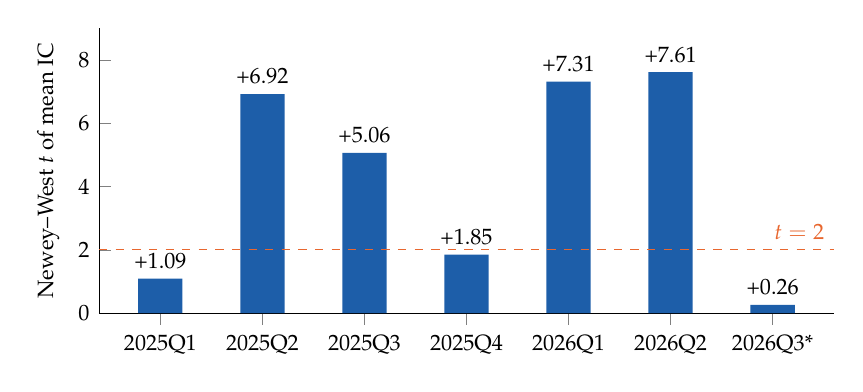
\begin{tikzpicture}
\begin{axis}[
  ybar,bar width=16pt,width=0.9\textwidth,height=5.2cm,
  symbolic x coords={2025Q1,2025Q2,2025Q3,2025Q4,2026Q1,2026Q2,2026Q3*},
  xtick=data,ymin=0,ymax=9,ylabel={Newey--West $t$ of mean IC},
  nodes near coords,every node near coord/.append style={font=\footnotesize},
  point meta=explicit symbolic,
  tick label style={font=\footnotesize},label style={font=\footnotesize},
  enlarge x limits=0.1,
  axis lines*=left,
]
\addplot[fill=linkblue,draw=none] coordinates {(2025Q1,1.09) [{+1.09}] (2025Q2,6.92) [{+6.92}] (2025Q3,5.06) [{+5.06}] (2025Q4,1.85) [{+1.85}] (2026Q1,7.31) [{+7.31}] (2026Q2,7.61) [{+7.61}] (2026Q3*,0.26) [{+0.26}]};
\draw[warm,dashed] (rel axis cs:0,0.2222) -- (rel axis cs:1,0.2222) node[above left,font=\footnotesize,warm] {$t=2$};
\end{axis}
\end{tikzpicture}
\caption{Newey--West $t$-statistic of the composite's mean daily IC by quarterly walk-forward block. The IC is positive in every block, but the first and last blocks carry almost no signal (IC 0.035 and 0.012) and 2025Q4 is also below $t=2$. The partial 2026Q4, 16 dates to 16 October 2026, is not one of the seven blocks and has a mean IC of $-0.266$.}\label{fig:quarters}
\end{figure}


The signal is positive in every quarterly block, but it is not uniform (Figure~\ref{fig:quarters}): three of the eight calendar quarters have a $t$-statistic below 2, and the first and the partial last carry almost no signal, with ICs of 0.035 and $-0.266$. Sign tests that do not depend on a long-run variance estimate confirm the signal and separate it from the money. Adjacent months share up to ten days of outcome overlap, so the binomial $p$-values are anti-conservative as printed; correcting them for the measured serial dependence of the monthly ICs (lags 1--3: 0.049, $-0.030$, 0.206, effective sample 15.4 months) leaves the signal test at $p=0.0037$ instead of $0.0022$, and on 45 non-overlapping ten-date blocks 38 are positive ($p<10^{-4}$). Under a symmetric null the probability of seven positive quarters out of eight is 0.035, and of at least 18 positive months out of 22 is 0.0022. For the book's net return, five positive quarters out of eight ($p=0.36$) and 14 positive months out of 22 ($p=0.14$) are not distinguishable from chance. The signal is robust to input noise and to total losses on the seven stocks delisted during the window \citep[cf.][]{shumway1997}, and it decays slowly with staleness: a ten-day-old forecast still has an IC of 0.052. The dividend check is a bound, not a measurement, because the calendar covers only eight tickers in the window.

\begin{table}[htbp]
\centering
\begin{threeparttable}
\caption{Robustness checks on the frozen composite}\label{tab:robust}
\small
\begin{tabularx}{\textwidth}{@{}R{2.9cm}R{3.6cm}L@{}}
\toprule
Check & Pre-specified criterion & Result \\
\midrule
Input noise (retrain; noise SD $=0.289m$, 3 seeds per level) & IC $\ge70\%$ of clean at $m=0.25$; positive in all seeds at $m=1$ & IC retains 98\%, 93\%, 85\% at $m=0.25,0.5,1$; minimum 0.078. Book net 0.073\%, 0.061\%, 0.035\% vs.\ 0.075\% per day. Pass \\
Stale signal (forecast of $d-k$ vs.\ outcome of $d$) & IC at $k=1\ge70\%$ of $k=0$; monotone decay & IC 0.0957, 0.0806, 0.0756, 0.0650, 0.0519 at $k=0,1,2,5,10$ (84\% at $k=1$). Book net 0.022\% at $k=1$, $-0.034\%$ at $k=2$. Pass for IC; book fragile \\
Total loss on delisted stocks & Sign of book net unchanged & 7 stocks delisted in the window; long positions lost entirely twice. Net 0.072\% vs.\ 0.075\%; difference $-0.003$\pp\ $[-0.010,0.000]$. Pass \\
Dividend gaps & Net moves by $<0.01$\pp & 132 of 45,636 stock-days excluded via calendar, which covers 8 tickers. Upper bound removing all next-day returns $>5$\pp from the universe mean: 0.069\% vs.\ 0.075\% $[-0.056,+0.047]$. Pass as a bound \\
Independent periods & IC $>0$ in $\ge6$ of 7 quarters and 80\% of months & IC $>0$ in 7 of 8 quarters and 18 of 22 months. Book net $>0$ in 5 of 8 quarters and 14 of 22 months. Pass; weak edges \\
Entry at next open & Net does not change sign & IC unchanged; net 0.031\% $[-0.057,+0.122]$ vs.\ 0.075\%. Pass, weaker \\
\bottomrule
\end{tabularx}
\begin{tablenotes}\footnotesize
\item Notes: Book results refer to the partial-adjustment book ($r=0.5$) with quoted-spread costs and 17\% borrow, kept for comparability with the earlier draft; the measured median of 25\% is used in Section~\ref{sec:money}, where carry enters linearly at about 0.0037\pp\ per day per percentage point and every figure in this table moves down by that amount. Intervals are 95\% block-bootstrap intervals. $m$ scales the noise added to every input.
\end{tablenotes}
\end{threeparttable}
\end{table}

\subsection{Sensitivity across declared grids}\label{sec:grids}

A single tuned optimum is weak evidence; a plateau is stronger. Table~\ref{tab:grids} collects the grids declared in the plans. On the fitting sample the ridge IC changes smoothly across a 300-fold range of the penalty, the elastic-net IC is flat around its optimum, and the net return declines monotonically with the horizon. On the real-time window the IC degrades gracefully with input noise and delay, whereas the net return is sensitive to every implementation parameter. Universe size was varied for the single feature A2 (top 100, 200 and 300) and, for the composite, through the thin universe of ranks 101--400; a top-50 universe was not run.

\begin{table}[htbp]
\centering
\begin{threeparttable}
\caption{Sensitivity across pre-declared grids}\label{tab:grids}
\small
\begin{tabularx}{\textwidth}{@{}R{3.1cm}R{3.5cm}L@{}}
\toprule
Parameter & Grid & Result \\
\midrule
\multicolumn{3}{@{}l}{\emph{Fitting sample (regenerated history, July 2022--December 2024)}} \\
Ridge penalty $\lambda_{\mathrm R}$ & 0.003, 0.01, 0.03, 0.1, 0.3, 1 & Mean IC from 0.1328 (best, 0.003) to 0.1167 (worst); smooth \\
Elastic-net penalty $\lambda_{\mathrm{EN}}$ & 0.0002 to 0.004 & Best 0.1326 at 0.001 \\
Horizon $H$ (quoted-spread book) & 10, 20, 40 days & Net 0.162\%, 0.141\%, 0.097\% per day; $H=10$ chosen \\
Adjustment speed $r$ & 1, 0.5, 0.33, 0.2, 0.1, 0.05 & Best 0.33 (flat costs), 0.5 (quoted spread), 0.2 (thin universe) \\
\addlinespace
\multicolumn{3}{@{}l}{\emph{Real-time window}} \\
Adjustment speed $r$ (flat costs) & 1 vs.\ 0.33 & Net $-0.065\%$ vs.\ $+0.030\%$ per day \\
Input noise $m$ & 0.25, 0.5, 1 & IC 98\%, 93\%, 85\% of clean; net 0.073\%, 0.061\%, 0.035\% \\
Signal delay $k$ & 0, 1, 2, 5, 10 days & IC 0.096 to 0.052; net 0.075\%, 0.022\%, $-0.034\%$ for $k\le2$ \\
Borrow rate (flat costs) & 17\%, 25\% & Net 0.030\% vs.\ $\approx0$ \\
Cost model & quoted spread, RUB 1 mn spread & Net 0.075\% vs.\ $-0.026\%$ \\
Universe, composite & top 100, ranks 101--400 & IC 0.096 vs.\ 0.129; best thin net 0.018\% \\
Universe, single feature A2 (flat costs; 10-day hold for top 100, 5-day for 200 and 300) & top 100, 200, 300 & $t=+5.6,+8.1,+8.6$; net by half $+0.006/+0.046$, $+0.014/+0.033$, $+0.013/+0.008$\% per day \\
\bottomrule
\end{tabularx}
\begin{tablenotes}\footnotesize
\item Notes: Fitting-sample values are optimistic because order-flow effects are larger on regenerated rows (Section~\ref{sec:regen}).
\end{tablenotes}
\end{threeparttable}
\end{table}

\subsection{Regenerated versus real-time history}\label{sec:regen}

Three observations show why the provenance rule matters. First, the A2 effect estimated on regenerated 2020--2024 rows is about twice its real-time size. Second, every quantity selected on the regenerated fitting sample is more optimistic than its real-time counterpart: the ridge component's IC on the fitting sample was 0.117--0.133 across the penalty grid, against 0.096 for the composite in real time, and the quoted-spread book earned 0.162\% per day on the fitting sample against 0.075\% in real time. Third, ten order-flow columns appeared to improve the price-based ensemble classifier on the long history; on the real-time window the AUC gain is $+0.002$ $[-0.017,+0.018]$ against a pre-specified threshold of $+0.016$, the 95th percentile of the procedure's own noise. A pre-registered round with within-date demeaned features and a demeaned placebo showed that the long-history gain was market timing. Kolmogorov--Smirnov distances between the distributions of 2024H2 and 2025H1 exceed 0.10 for A2 (0.112), five-day A2 (0.137) and the spread ratio (0.140).

A within-date permutation placebo cannot catch this problem: it preserves the date-level moments of the features, so any market-timing component survives the permutation. Demeaned features and demeaned placebos are needed.

Regeneration and calendar time are confounded in our data: the regenerated rows are exactly the 2020--2024 rows. The halving of the A2 effect is consistent with a regeneration artefact, with genuine decay of the effect, or with both. The rule protects verdicts against either explanation.

\subsection{What does not add}\label{sec:noadd}

Several extensions raised the composite's IC or seemed promising but did not change its economics.
\begin{itemize}
\item \textbf{Momentum.} The 256-day momentum signal is confirmed on independent price history (2021--2024: IC 0.0380, $t=2.56$, 919 dates). Added to the composite it raises the IC by 0.0105 ($t=2.39$), but the net gain at 25\% borrow is 0.008\pp\ per day, identical to that of a placebo with shuffled momentum.
\item \textbf{Features proposed by language models.} Three local language models proposed 75 ideas, of which five were implementable (pre-dividend flow asymmetry, PageRank of imbalance correlations, Legendre-polynomial profile shapes, closing-auction imbalance for next-open entry, entropy of turnover and depth). The IC increment is 0.0016 $[-0.0020,+0.0057]$.
\item \textbf{Transformations.} A library of 100 transformations of the 16 strongest features (five-day means, $z$-scores, changes, liquidity-tercile ranks, lags and 20 interactions) produced 0 of 100 hits at $p\le0.00052$ ($M_{\mathrm{eff}}=95.5$), 0 of 5 placebo hits, and 4 rows with $p<0.05$ against 5 expected by chance.
\item \textbf{Moderators.} Among 105 candidate moderators, two nominal hits (both forms of agreement between level asymmetry and A2) showed an IC of 0.149 in the top third versus 0.060 in the bottom third ($t=5.08$). But the control moderator ``absolute size of the forecast itself'' produced a larger difference (0.142), and within strata of equal forecast confidence the effect is 0.015 ($t=0.81$). Subgroups with wider predictor dispersion mechanically show higher correlations; there was no discovery.
\item \textbf{A pretrained foundation model.} Zero-shot TimesFM forecasts \citep{das2024} on 256-day abnormal-return histories (40,851 forecasts) added nothing beyond the composite (0 of 3 rows). A placebo fed another stock's covariates performed as well as the real version (IC 0.0825 vs.\ 0.0814), so the model does not use the covariates; its forecast correlates 0.65 with 12-month momentum. Eleven further uses (102,325 forecasts) also failed, although its 80\% prediction intervals were well calibrated (coverage 0.80--0.82). This matches \citet{rahimikia2025} and \citet{alonso2026}.
\end{itemize}

\section{Results II: monetization}\label{sec:money}

\subsection{Net returns of the books}\label{sec:book}

Table~\ref{tab:books} and Figure~\ref{fig:books} report the books. Under the flat 0.15\% tariff, daily rebalancing loses 0.065\% per day; partial adjustment with $r=0.33$ lifts this by 0.095\pp\ $[+0.059,+0.131]$ to a gain of 0.030\% per day (about 7.5\% a year), which falls to zero at 25\% borrow. The signal and execution criteria of Section~\ref{sec:criteria} are met, the economic criterion fails. Two books are referred to from here on and the distinction matters for every rate threshold below: the \emph{published book}, $r=0.5$ under quoted-spread costs, which is the gate book of Table~\ref{tab:books} and earns 0.0753\% per day at 17\% borrow; and the \emph{frozen book}, $r=0.33$, which is the configuration whose models are frozen for the forward test and which earns 0.0679\% per day at the same carry. The borrow curve in the next paragraphs is the frozen book, because that is the configuration the programme will actually read forward.

A later plan re-evaluated the economics with quoted-spread costs, choosing the horizon on the fitting sample. On the real-time window the main book earns 0.0753\% per day with a 95\% interval of $[-0.005\%,+0.163\%]$ and a Newey--West $t$ of 1.71; both halves are positive (0.066\% and 0.087\%), the five placebo books lose 0.34--0.40\% per day, almost all of it cost. A placebo forecast has no cross-sectional information, its daily IC sits between -0.004 and +0.005, so its book turns the same turnover against a zero edge and its loss measures the cost model rather than the absence of signal. The book-level placebo criterion is close to mechanical for that reason, and the informative placebo comparison is at the level of the forecast, where it is reported. The gate fails narrowly. A one-sided test would reject zero at 5\%, but the gate was specified as two-sided and is not altered after the fact. With the spread for a RUB 1 million order the net return is negative. At quoted-spread costs partial adjustment beats daily rebalancing (0.048\% per day) by 0.027\pp\ $[-0.000,+0.055]$, a weaker execution gain than under the flat tariff.

\paragraph{At the measured borrow rate.} The 0.0753\% figure above is charged at 17\% a year, a secondary quote. The broker's contractual short terms were measured for the admitted universe after this run: 72 of the 99 names resolve, 68 are short-enabled, and the annual rate ranges from 20.0\% to 125.0\% with median 25.0\%, quartiles 22.0\% and 36.9\% --- no admitted name is available at 17\%. Carry enters equation~(\ref{eq:net}) linearly, so the whole curve follows from the same run at 0.0037\pp\ per day per percentage point of annual rate. The main book is then $+0.0679$\% per day at 17\%, $+0.0383$\% at the measured median of 25\% ($t=0.89$, $[-0.040,+0.122]$), $+0.0199$\% at 30\% ($t=0.46$) and $-0.006$\% at the upper quartile of 36.9\%. Three rate thresholds matter and they belong to two different books. On the curve above, which is the frozen $r=0.33$ book, the net falls by 0.00370--0.00375\pp\ per day per point of annual rate --- an implied short exposure of 0.93 rather than 0.95 --- so the book breaks even at 35.3\% and clears the lower end of the policy band (14\% a year) only below 20.3\%. The published $r=0.5$ book, at 0.0753\% per day, breaks even at 36.8\%; that is the figure the earlier draft carried, and it is stated here as the $r=0.5$ anchor rather than as a property of the curve. The cheapest rate the broker offers on any admitted name is 20.0\%, so the whole survivable range is a fraction of one percentage point wide and no name in the universe sits inside it. Under the flat tariff of the live account the same book nets 0.0298\% at 17\% and nothing at 25\%. Measured against the policy rate rather than against zero, the book at the median carry earns 0.0383\% per day against 0.0556--0.0833\% that the same capital could earn risk-free, i.e.\ an excess return of between $-0.017$ and $-0.045$\pp\ per day; the information ratio of 1.56 is a statement about dispersion, not about that difference.Every economic reading in this paper that used 17\% is therefore an upper bound; the measured median is the number we report first, and it lowers the economics at every horizon, never raises them. Two clarifications about what the grid does and does not contain. The step from 0.0753\% to 0.0679\% at 17\% is the change of the adjustment speed from $r=0.5$ to the frozen $r=0.33$, not a dividend adjustment: the dividend term is not in the book at all and is reported separately as a bound below, so the grid is optimistic by 0.0038--0.0126\% per day relative to a full accounting. And the grid uses the measured rate but not the measured per-name assignment: the median is applied to the whole short leg, whereas the rates are per name and the short quintile is not a random sample of the universe. The endogeneity of the fee, if it exists, biases the median figure upward, and the mean of 32.1\% costs a further 0.0271\% per day.

\paragraph{The cost model is a decision variable, not a detail.} Two cost models are carried through every table and they can disagree in sign, so neither is decorative. The composite book turns over 0.63 of its notional a day and the momentum sleeve 0.16, a factor of four; quoted half-spreads average 8.6--9.5\bp\ per side for these names, while the live retail tariff is a flat 15\bp. Quoted spreads therefore flatter the high-turnover leg and the flat tariff penalizes it. The registered momentum contrast illustrates the size of the effect: $+0.0194$\% per day under quoted spreads against $-0.0102$\% under the flat tariff of the live account. Every contrast whose sign moves between the two is marked as such, and because the live account pays the flat tariff, the flat read is the conservative one wherever the two disagree.

\paragraph{The short leg and the Sharpe ratio.} The gross return is concentrated where the borrow cost is: over the quoted-spread window the long leg earns 0.0236\% per day and the short leg 0.2002\%, so the short side carries 89.5\% of the gross 0.2238\%. The book's beta to the equal-weighted universe is $-0.269$, and in a window in which the universe fell it was net short: hedging that exposure costs 0.0213\% per day, exactly $|\beta|\cdot20\%/252$, and leaves $+0.0538$\% (Newey--West $t=1.49$). The beta-hedged figure, not the raw 0.075\%, is the headline of this section. Two further corrections apply to the short leg and neither requires new data. First, dividends: the book is charged no dividend on the names it is short, and the raw close-to-close return already reflects the ex-date gap, so the net is overstated by $0.96\cdot\Delta y/252$ where $\Delta y$ is the gap between the dividend yields of the long and the short leg. With the top-100 yield at 3.3\% the one-sided worst case, in which the long leg earns no dividend at all, is 0.0126\% per day, 17\% of the unhedged net; a realistic gap of 1 percentage point is 0.0038\%. Second, the Sharpe ratio: 1.56 is computed on 0.766\% daily volatility without adjustment for serial dependence. With the book's own autocorrelation factor of 1.87 the same series gives an annualized Sharpe ratio of 1.14, and with the Bartlett-weighted factor of 1.51 it gives 1.27. The deflated probabilities of Table~\ref{tab:dsr} already use the 1.87 variant; the undeflated headline does not.

\begin{table}[htbp]
\centering
\begin{threeparttable}
\caption{Net returns of composite books on the real-time window}\label{tab:books}
\small
\begin{tabularx}{\textwidth}{@{}Lrcr@{}}
\toprule
Book & Net, \% per day & 95\% interval & Approx.\ \% p.a. \\
\midrule
\multicolumn{4}{@{}l}{\emph{Top 100, flat 0.15\% per side, 17\% borrow (comparable to the earlier draft; the measured curve is in the text)}} \\
Daily rebalancing & $-0.065$ & $[-0.149,+0.027]$ & $-16$ \\
Partial adjustment, $r=0.33$ & $+0.030$ & $[-0.048,+0.114]$ & $+7.5$ \\
\quad same, 25\% borrow & $\approx0$ & & $\approx0$ \\
\addlinespace
\multicolumn{4}{@{}l}{\emph{Top 100, quoted-spread costs, $r=0.5$, $H=10$, 17\% borrow (measured curve in the text)}} \\
Main book (gate) & $+0.0753$ & $[-0.005,+0.163]$ & $+19$ \\
\quad entry at next open & $+0.031$ & $[-0.057,+0.122]$ & $+8$ \\
\quad spread for a $\approx$RUB 1 mn order & $-0.026$ & $[-0.109,+0.062]$ & $-7$ \\
\quad signal delayed 1 / 2 days & $+0.022$ / $-0.034$ & & \\
\quad beta-hedged to the universe & $+0.0538$ & $[-0.012,+0.125]$ & $+14$ \\
\quad sector-neutral forecast & $+0.0446$ & $[-0.027,+0.126]$ & $+11$ \\
\quad plus five LLM-proposed features & $+0.0817$ & $[+0.006,+0.166]$ & $+21$ \\
\addlinespace
\multicolumn{4}{@{}l}{\emph{Thin universe (ranks 101--400), quoted-spread costs, $r=0.2$}} \\
Long--short, 25\% borrow & $+0.0174$ & $[-0.023,+0.063]$ & $+4.4$ \\
Long-only vs.\ equal-weighted universe & $+0.0184$ & $[-0.004,+0.045]$ & $+4.6$ \\
\bottomrule
\end{tabularx}
\begin{tablenotes}\footnotesize
\item Notes: Annualized figures are the daily mean times 252, rounded. The main book's Newey--West $t$ is 1.71 and its annualized Sharpe ratio 1.56 over 457 days. The extended book's improvement over the main book is $+0.007$\pp\ $[-0.011,+0.025]$, i.e.\ noise. The policy rate ranged from 14\% to 21\% a year (0.056--0.083\% per trading day). Beta-hedged: Newey--West $t=1.49$.
\end{tablenotes}
\end{threeparttable}
\end{table}

\begin{figure}[htbp]
\centering
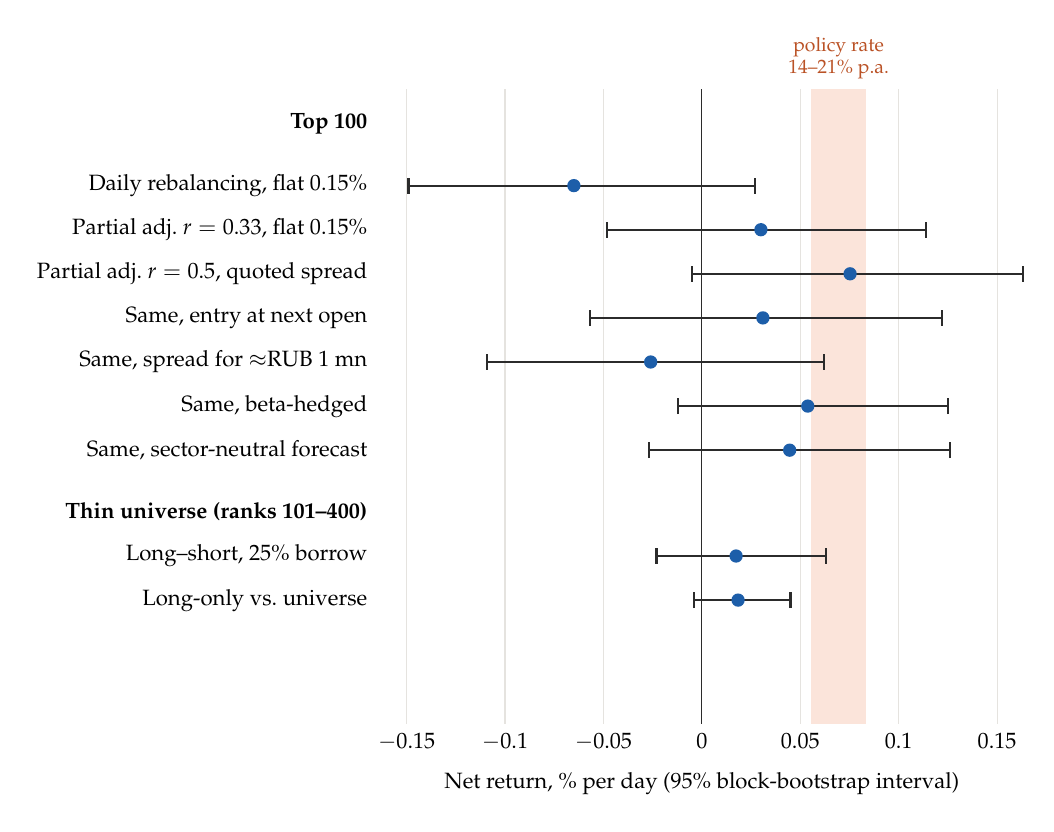
\begin{tikzpicture}[x=25cm,y=0.56cm,font=\footnotesize]
\fill[warm!18] (0.0556,-1.2) rectangle (0.0833,13.2);
\node[warm!80!black,font=\scriptsize,align=center] at (0.0695,13.9) {policy rate\\14--21\% p.a.};
\draw[grey!40] (-0.15,-1.2) -- (-0.15,13.2);
\foreach \v in {-0.15,-0.10,-0.05,0,0.05,0.10,0.15}{
  \draw[grey!40] (\v,-1.2) -- (\v,13.2);
  \node[below] at (\v,-1.2) {\pgfmathprintnumber[fixed,precision=2]{\v}};
}
\draw[ink] (0,-1.2) -- (0,13.2);
\newcommand{\bookrow}[5]{
  \draw[ink,line width=0.8pt] (#3,#1) -- (#4,#1);
  \draw[ink,line width=0.8pt] (#3,#1-0.18) -- (#3,#1+0.18);
  \draw[ink,line width=0.8pt] (#4,#1-0.18) -- (#4,#1+0.18);
  \fill[linkblue] (#2,#1) circle (2.4pt);
  \node[anchor=east] at (-0.165,#1) {#5};
}
\node[anchor=east,font=\footnotesize\bfseries] at (-0.165,12.4) {Top 100};
\bookrow{11}{-0.065}{-0.149}{0.027}{Daily rebalancing, flat 0.15\%}
\bookrow{10}{0.030}{-0.048}{0.114}{Partial adj.\ $r=0.33$, flat 0.15\%}
\bookrow{9}{0.0753}{-0.005}{0.163}{Partial adj.\ $r=0.5$, quoted spread}
\bookrow{8}{0.031}{-0.057}{0.122}{Same, entry at next open}
\bookrow{7}{-0.026}{-0.109}{0.062}{Same, spread for $\approx$RUB 1 mn}
\bookrow{6}{0.0538}{-0.012}{0.125}{Same, beta-hedged}
\bookrow{5}{0.0446}{-0.027}{0.126}{Same, sector-neutral forecast}
\node[anchor=east,font=\footnotesize\bfseries] at (-0.165,3.6) {Thin universe (ranks 101--400)};
\bookrow{2.6}{0.0174}{-0.023}{0.063}{Long--short, 25\% borrow}
\bookrow{1.6}{0.0184}{-0.004}{0.045}{Long-only vs.\ universe}
\node[below=14pt] at (0,-1.2) {Net return, \% per day (95\% block-bootstrap interval)};
\end{tikzpicture}
\caption{Net daily return of composite books with 95\% block-bootstrap intervals. Every interval shown includes zero. The shaded band shows the policy rate (14--21\% a year) expressed per trading day, for scale. The extended-feature book (Table~\ref{tab:books}) is not shown; its gain over the main book is noise.}\label{fig:books}
\end{figure}


\subsection{Where monetization is lost}

\paragraph{Turnover.} Daily rebalancing of a 10-day forecast is wasteful: moving from $r=1$ to $r=0.33$ improves the flat-cost book by about 0.095\pp\ per day. This is the mechanism of \citet{garleanu2013} and is consistent with \citet{novymarx2016}.

\paragraph{Delay.} Figure~\ref{fig:delay} shows the central asymmetry of the paper. The IC of a one-day-old forecast retains 84\% of its value and a ten-day-old forecast 54\%. The book's net return retains 29\% with a one-day delay and turns negative with a two-day delay. Entering at the next open instead of the close costs 0.044\pp\ per day. The part of the predictability that covers costs is concentrated in the first one or two days of the horizon, while the slower part, which keeps the 10-day IC high, does not pay for the trading it requires.

\begin{figure}[htbp]
\centering
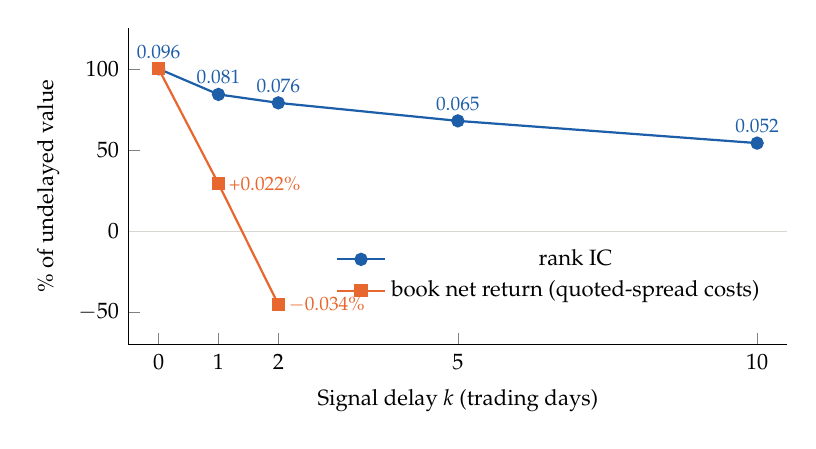
\begin{tikzpicture}
\begin{axis}[
  width=0.82\textwidth,height=5.6cm,
  xmin=-0.5,xmax=10.5,ymin=-70,ymax=125,
  xtick={0,1,2,5,10},ytick={-50,0,50,100},
  xlabel={Signal delay $k$ (trading days)},ylabel={\% of undelayed value},
  tick label style={font=\footnotesize},label style={font=\footnotesize},
  axis lines*=left,
  legend style={font=\footnotesize,at={(0.98,0.22)},anchor=east,draw=none,fill=none},
  point meta=explicit symbolic,
  every node near coord/.append style={font=\scriptsize},
]
\draw[grey!60] (axis cs:-0.5,0) -- (axis cs:10.5,0);
\addplot[linkblue,thick,mark=*,nodes near coords,nodes near coords align={above}] coordinates {(0,100) [{0.096}] (1,84.2) [{0.081}] (2,79.0) [{0.076}] (5,67.9) [{0.065}] (10,54.2) [{0.052}]};
\addplot[warm,thick,mark=square*,nodes near coords,nodes near coords align={right}] coordinates {(0,100) [{}] (1,29.2) [{+0.022\%}] (2,-45.2) [{$-0.034\%$}]};
\legend{rank IC,book net return (quoted-spread costs)}
\end{axis}
\end{tikzpicture}
\caption{Signal versus money under delay. Rank IC of a forecast made $k$ trading days earlier (blue) and net daily return of the partial-adjustment book under quoted-spread costs when the signal is delayed (orange), both as a share of their undelayed values (IC 0.0957; net 0.075\% per day). Labels give raw values.}\label{fig:delay}
\end{figure}


\paragraph{Latency.} The protocol implies a twenty-minute window: features from bars ending at 18:30, orders into the 18:50 closing auction. Two different things are called a timestamp here and only one of them is measured. The data carry \texttt{SYSTIME}, the exchange's record stamp, which is provenance and not delivery; and the pipeline that produced this paper writes the file for date $d$ at 00:20 on $d+1$ --- the daily fetch job runs at 00:20, and each of the last ten raw files carries that arrival time to the minute. Nothing in the programme has ever executed in the same evening as the signal. Whether a subscriber's feed delivers the 18:25--18:30 bar before 18:50 is therefore untested here, and it is the first measurement a pilot should make: if delivery lags by more than twenty minutes the same-evening construction is unavailable, and the implementable variant is the next open, which costs 59\% of the net return.

\paragraph{The short leg.} A decisive test of a different construction, an ensemble of gradient-boosted trees and a logit on ten demeaned order-flow columns, produced a top-minus-bottom decile spread in 10-day abnormal returns of 0.952\% per date net of a 0.30\% round-trip cost (interval $[0.311\%,1.537\%]$, Newey--West $t=2.95$). The entire effect sits in the short leg: the long-only version earns $-0.16\%$. Holding the short leg for ten trading days at 17--25\% annual borrow costs roughly 0.67--0.99\%, most or all of the point estimate (our illustration; the test's cost assumption did not include borrow). This matches the pattern in \citet{muravyev2025}.

\paragraph{Market exposure.} The main book's beta to the equal-weighted universe is $-0.269$: during a falling market it was net short. After hedging this exposure the net return is 0.0538\% per day ($t=1.49$).

\paragraph{Time variation.} The signal is weak in the first and last quarters. In an exploratory analysis of 45 state variables, the composite's IC is 0.139 when the RVI volatility index is below its trailing median and 0.045 when it is above (circular-shift $p=0.0024$); the effect sits in book-shape features rather than A2. Trading only in calm states would add about 2\% a year, the monetary difference is not significant ($p=0.148$), and the result does not survive the stricter threshold of the next wave.

\paragraph{Risk profile.} A Sharpe ratio is not a sufficient summary of a series with skewness $-1.52$ and excess kurtosis 13.4, so the risk of the book is reported directly. Over the 457 dates the gate book compounds to $+39.0\%$ with a maximum drawdown of $-18.2\%$, from the peak of 16 July 2026 to the trough of 4 August 2026: three weeks give back more than half of the cumulative result. Months are 22, of which 8 are negative (36\%), the worst $-8.6\%$ and the best $+11.7\%$. The one-day 99\% loss, measured historically, is $-1.74\%$; the mean of the worst 1\% of days is $-3.63\%$; a normal approximation on the same mean and variance gives $-1.86\%$ and the Cornish--Fisher correction on the same moments gives $-4.29\%$. The last figure is the one a desk should carry: the Gaussian rule understates a bad day by a factor of 2.3, and one such day costs about 57 days of expected net return. At the measured median carry the same drawdown is $-18.5\%$ and the terminal equity $1.21$ instead of $1.39$, because the drawdown is a fast event and the carry is a slow one. The sector-neutral book has a drawdown of $-16.2\%$, 99\% historical loss $-1.60\%$ and Cornish--Fisher $-3.75\%$; at 25\% carry it earns 0.0141\% per day, 3.6\% a year, which retires the sector-neutral variant on economics alone.

\paragraph{Capacity.} The book holds forty positions with inverse-volatility weights, so capacity is set by the spread at the order size, not by the forecast. The RUB 1 million stress model is the only size-dependent measurement in the paper, and at that size the book already loses 0.026\% per day, $-6.4$\% a year. A comfortable ceiling is therefore tens of millions of roubles of gross exposure, not hundreds: at 10--20 million roubles per leg the expected net is 7.5--15 thousand roubles a day against a daily standard deviation of roughly 90 thousand on the same notional, a signal-to-noise ratio near 0.08 per day. This is the class of a personal account run by someone who values the research, not a product for an allocator, and it is one more reason the paper positions itself as an audit.

\subsection{Deflation and track-record length}

The main book's annualized Sharpe ratio of 1.56 over 457 days (skewness $-1.52$, kurtosis 16.4) has a probabilistic Sharpe ratio of 0.973 against zero. Table~\ref{tab:dsr} shows how quickly this evidence weakens once selection is accounted for. With ten trials, the expected maximum Sharpe ratio of skill-less strategies over 1.81 years is 1.17 and the deflated probability falls to 0.685; with 100 trials the expected maximum (1.88) exceeds the observed value and the deflated probability is 0.346. The null variance $1/T$ ignores the autocorrelation of daily book returns; correcting it (factor 1.87) lowers the deflated probabilities further, to 0.480 at ten trials and 0.106 at one hundred. The program's registry counts 41 attempts for the first model alone and many more across directions, so the relevant column is not the first. The conclusion about the signal is unaffected: the IC was tested against placebos, not selected as the best of $N$ books.

\begin{table}[htbp]
\centering
\begin{threeparttable}
\caption{Deflation of the main book's Sharpe ratio}\label{tab:dsr}
\small
\begin{tabularx}{\textwidth}{@{}Lrrrrrr@{}}
\toprule
Number of trials $N$ & 1 & 10 & 50 & 100 & 300 & 800 \\
\midrule
Expected max.\ annual Sharpe without skill & 0 & 1.17 & 1.69 & 1.88 & 2.15 & 2.37 \\
Years at which this equals the observed 1.56 & --- & 1.02 & 2.14 & 2.64 & 3.46 & 4.20 \\
Deflated probability, null variance $1/T$ & 0.973 & 0.685 & 0.435 & 0.346 & 0.233 & 0.158 \\
Deflated probability, autocorrelation-adjusted & --- & 0.480 & 0.176 & 0.106 & 0.044 & 0.019 \\
\bottomrule
\end{tabularx}
\begin{tablenotes}\footnotesize
\item Notes: Quoted-spread costs, $r=0.5$, 17\% borrow, 457 trading days (1.81 years). Expected maxima use $V=1/T$ \citep{bailey2014dsr}; the years row is the track-record length at which the expected maximum of $N$ skill-less trials equals the observed Sharpe ratio (deflated probability 0.5). The adjusted row inflates $V$ by 1.87, the autocorrelation factor of the daily series. The pre-specified reading rule was that a deflated probability below 0.95 at $N=10$ makes the book indistinguishable from the best of ten skill-less books.
\end{tablenotes}
\end{threeparttable}
\end{table}

\section{Economic uncertainty}\label{sec:uncertainty}

The forecasting result rests on measured quantities. The economic result does not. This section separates the two, states what each assumption is worth, and specifies the analyses that would reduce the uncertainty.

\subsection{Measured, bounded and assumed inputs}

Table~\ref{tab:inputs} classifies every input to the net return of the main book. The quoted spread, the book's market exposure and now the short-borrow fee are measured; the delisting and dividend inputs are bounded by deliberately pessimistic checks; the commission, the price impact beyond the quoted spread, the execution time and above all the borrow availability by date are assumed.

\begin{table}[htbp]
\centering
\caption{Inputs to the economic result: measured, bounded or assumed}\label{tab:inputs}
\small
\begin{tabularx}{\textwidth}{@{}R{2.6cm}R{1.8cm}R{4.4cm}L@{}}
\toprule
Input & Status & Value used & Effect on net return (\% per day) \\
\midrule
Quoted spread & Measured & Half the best-quote spread, per stock-day (AlgoPack \texttt{obstats}) & Main book $+0.075$ \\
Market exposure & Measured & Beta $-0.269$ to the universe & Hedged $+0.054$ ($t=1.49$) \\
Delisting proceeds & Bounded & Total loss on 7 delisted stocks & $+0.072$ \\
Dividend gaps & Bounded & Calendar covers 8 tickers; outlier bound & $+0.069$ \\
Commission & Assumed & 0.15\% per side (flat) or 0.05\% plus spread & Flat-cost partial book $+0.030$ \\
Impact beyond the touch & Proxied & Half the spread for $\approx$RUB 1 mn & $-0.026$ \\
Execution time & Assumed & Close of signal day via closing auction & Next open $+0.031$; 1-day delay $+0.022$; 2-day $-0.034$ \\
Borrow fee & Measured & 25.0\% a year median (20.0--125.0\%, quartiles 22.0 and 36.9), 72 of 99 names resolved & Main book $+0.0679$ at 17\%, $+0.0383$ at 25\%, $+0.0199$ at 30\%, $-0.006$ at 36.9\%; see Section~\ref{sec:borrow} \\
Borrow availability & Not measured & All short-leg names (top 100) assumed borrowable & Unknown; 10 of 60 thin names shortable \\
Rebalancing rule & Chosen on fitting & $r=0.5$ (spread), 0.33 (flat) & Daily rebalancing (flat) $-0.065$ \\
\bottomrule
\end{tabularx}
\end{table}

\subsection{Borrow: break-even rates and availability}\label{sec:borrow}

Because the book is dollar-neutral, its short exposure is close to one unit of capital, so each additional percentage point of annual borrow costs about $1/252\approx0.004$\pp\ per day (equation~\ref{eq:net}); the measured coefficient of the curve is 0.00370--0.00375, i.e.\ a short exposure of 0.93. The flat-cost book's decline from 0.030\% at 17\% to roughly zero at 25\% matches this arithmetic. Applied to the quoted-spread book, the same arithmetic gives 0.0679\% per day at 17\%, 0.0383\% at 25\%, 0.0199\% at 30\% and $-0.006$\% at 36.9\%, so this book breaks even at 35.3\% a year and clears the lower end of the policy band only below 20.3\%; the published $r=0.5$ book, which earns 0.0753\% at 17\%, breaks even at 36.8\%. For the flat-cost book the break-even rate is about 25\%. These are derivations from the reported results and they ignore estimation error, but the earlier caveat that the fee was unmeasured no longer applies.

The fee is now measured at the source, through the broker's contract-terms endpoint for the admitted universe: of 99 names, 72 resolve as shares and 68 are short-enabled, with the annual rate running from 20.0\% to 125.0\%, median 25.0\%, quartiles 22.0\% and 36.9\%, and a mean of 32.1\%. The 17\% used as the base of the earlier draft is below the cheapest quartile and below every individual name; 25\%, previously described as a stress, is the median. Nothing in the programme becomes more favourable under the correction, and three of its registered verdicts were read on a rate the market does not offer.

Availability is a separate problem and remains unmeasured. The rule assumes that every name in the short quintile can be borrowed every day. We now record the contractual terms and the short flag daily through the broker's terms endpoint, which is instrument metadata and therefore available historically from the recording date forward, but the broker exposes no series of borrow limits, so the intraday availability of a name is still an assumption. Among the 60 thin stocks we checked by hand, only 10 could be shorted. If availability is correlated with the forecast, for example if the most negatively forecast names are also the hardest to borrow, the short leg's measured return overstates what can be captured, which is the mechanism documented by \citet{muravyev2025}. The decile-spread evidence, in which the entire effect sits in the short leg, makes this concern concrete.

\subsection{The portfolio mapping is a design choice}\label{sec:mapping}

All books in Table~\ref{tab:books} map the forecast into equal-gross long and short quintiles with inverse-volatility weights. That mapping is conventional, not optimal. \citet{jacobs1998} show that the optimal long--short portfolio integrates both legs rather than combining two separate sorts, and \citet{grinold2000b} quantify how the efficiency gain from shorting depends on constraints and costs. When the short leg is expensive and partly unavailable, a scaled-down or borrow-constrained short leg, or a long-only implementation, may dominate. The long-only evidence we have is mixed: for single features, long top-quintile books against the universe failed in all 28 confirmatory real-time rows; in the thin universe the long-only composite book earns 0.0184\% per day with an interval that includes zero; and for the decile-spread ensemble the long leg alone loses money. A long-only top-100 composite book was not run.

\subsection{What the sample can and cannot say}

A non-significant net return is not evidence of a zero net return. Define a smallest effect size of interest $\delta$ for the net return of an implementable book. For an investor whose capital could otherwise earn the policy rate, a natural choice is the lower end of that rate, 14\% a year or $\delta\approx0.056\%$ per day. The main book's standard error is about 0.043\pp\ per day (from its bootstrap interval). Its 90\% interval, $[0.005\%,0.146\%]$, contains values well above $\delta$, so an equivalence test \citep{lakens2017} cannot conclude that the net return is negligible; its 95\% interval contains zero, so the pre-specified test cannot conclude that it is positive. The data are inconclusive.

Assuming the daily variance and autocorrelation stay as observed, the sample size for a two-sided test at 5\% with 80\% power follows from one formula, $T=\big[(z_{0.975}+z_{0.80})\,\sigma_{\mathrm{LR}}/\delta\big]^2$ with $z_{0.975}+z_{0.80}=2.80$ and $\sigma_{\mathrm{LR}}$ the autocorrelation-adjusted daily volatility of the book, 0.941\% against the plain 0.766\%. For $\delta=0.0753$ that gives 1,226 trading days (4.9 years); for $\delta=0.056$, the lower end of the policy rate, 2,215 days (8.8 years). The earlier draft printed 1,160 and 2,300 without the formula or $\sigma_{\mathrm{LR}}$; both follow from the same expression to within 6\%, and the inputs are now stated. These rough calculations show the order of magnitude: the economic question cannot be settled on a 1.8-year window.

The frozen forward test (60 dates) cannot settle it either, and its power against the quantity it is asked to confirm is the one number the protocol was missing. Over 60 dates the standard error of the book's mean net return would be about 0.12\pp\ per day, which is uninformative. The standard error of the mean IC would be about 0.045, so an IC of 0.096 would produce $t\approx2.1$. For the confirmation rule itself --- the 95\% interval of the IC increment above zero --- the increment's Newey--West standard error over 450 dates is 0.0147, which scales to 0.0402 over 60 dates because the series is autocorrelated (variance factor 5.3, effective sample 84.7 dates). The minimum detectable increment is then 0.0787, more than twice the observed 0.0368, and the power of the rule against an effect of the observed size is \textbf{15\%}. Reaching 80\% power takes 561 dates at the interval rule, 1,056 at $|t|\ge3.0$ and 1,317 at $|t|\ge3.45$. A block bootstrap of the 60-date mean (10-date blocks, 4,000 draws) reproduces the standard error, 0.0408 against 0.0402. The forward read is therefore a falsification test, not a confirmation test, and Section~\ref{sec:criteria} and the abstract say so. Measuring the borrow fee was worth more than additional forward dates; measuring availability still is.

\subsection{Pre-specified extensions}\label{sec:extensions}

The following analyses address the main open questions. E1 has since been run and is reported below; the other four have not been run. Each is listed with its gate so that, when run, it is evaluated against criteria fixed in advance; they form one family of five. Because the real-time window has been used, any positive result on it can only be a lead; confirmation requires forward data.
\begin{description}[leftmargin=2.2em,style=nextline]
\item[E1. Information beyond momentum.] \emph{Run 2026-10-29; null.} The composite and a 256-day momentum rank were put through the same partial-adjustment book with the same costs and carry, together with the composite's residual after projection on the momentum rank. At the measured median carry of 25\% the composite nets 0.0383\% per day, the momentum sleeve 0.0189\% and the residual 0.0373\%; the registered contrast, composite minus momentum, is $+0.0194$\% per day with a Newey--West $t$ of 0.44 and a block-bootstrap interval $[-0.0739,+0.0974]$, and residual minus momentum is $+0.0184$\% with an interval that also contains zero. Both registered criteria fail: the contrast is not separated from zero, and at the higher adjustment speed its halves disagree in sign. At the level of ranking the composite keeps 91\% of its IC after the momentum span is removed (0.0869, $t=7.33$), so it is not a momentum proxy; at the level of money the two are indistinguishable. With the flat 0.15\% tariff of the live account the contrast turns $-0.0102$\% per day, so its sign depends on the cost model --- a further reason to report both.
\item[E2. Long-only implementation.] Top-quintile composite book on the top 100 against the equal-weighted universe, quoted-spread costs, no borrow; gate: net interval above zero in both halves, placebo books non-positive.
\item[E3. Borrow-feasible short leg.] Short only names with recorded availability on the date, charged at the recorded fee; the fee is now recorded daily, the availability by date still is not.
\item[E4. Hold bands.] Enter the top (bottom) quintile and exit only when a name leaves the top (bottom) 40\%, the buy/hold spread of \citet{novymarx2016}.
\item[E5. Scaled short exposure.] Short-leg scale chosen on the fitting sample from a declared grid, following \citet{jacobs1998}.
\end{description}

\subsection{A second real-time window}\label{sec:realtime2}

The window used in this paper has been read many times, by this study and by the studies before it, and rule (ii) of Section~\ref{sec:protocol} makes every result on it a lead. A resubmission that repeats the same window would inherit the same defect, so the protocol designates a second one now, before it is read.

\emph{Dates.} Feature dates from 19 October 2026 onward: the first trading date after 16 October 2026, the last date of the spent window. No date in this window has been used for any verdict, plan or exploratory screen in this programme.

\emph{Frozen contents.} The two model files with their SHA-256 hashes, the trade rates (0.33 flat, 0.50 quoted), the horizons, the three cost models, the two carry scenarios, the quintile mapping, and the five criteria of Section~\ref{sec:criteria} with the corrected power rule of Section~\ref{sec:uncertainty}. The momentum sleeve is a co-primary rather than a robustness check, because the first window established that it nets at least as much as the composite: the second window measures both books under identical machinery.

\emph{Reading rule.} One reading, at 561 dates, the horizon at which the increment rule reaches 80\% power against the effect observed in the first window; the first date at which that count is complete is about November 2028 at the current rate of accrual. An interim reading at 60 dates is permitted only as a falsification check --- a negative sign, or an interval excluding the first-window effect, retires the lead --- and never as confirmation. No date is added after the reading, no window is extended, and no parameter is recomputed.

\emph{What is still missing.} The fee is recorded daily from 29 October 2026; availability by date is not, so a short-feasible reading (E3) remains open. A single-author programme cannot produce the external replication that would settle the question independently of its author, and the second window does not claim to.

\emph{Registration.} The protocol of this subsection, with the file hashes, the criteria and the two reading dates, is deposited before the first reading with a public timestamping service and mirrored in the repository; the version of record is the deposited one, and later edits are recorded as amendments with their dates.

\section{Secondary results and exploratory leads}\label{sec:secondary}

\paragraph{Execution timing (passed).} Using quoted best-quote spreads for 244 stocks over 461 days, the cheapest half-hour window is almost never the opening one. Relative to trading at the open, choosing a window by each stock's own trailing spread profile saves 0.25\bp\ per side for the tightest-spread third, 2.0\bp\ for the middle third and 12.9\bp\ for the widest third. A control using a neighbour's profile is positive in all groups, so the gain comes from a universal rule (``do not trade at the open''); the stock-specific window adds 0.2\bp. These are quoted spreads, not executed prices.

\paragraph{Leads.} Table~\ref{tab:leads} lists the five leads. None is a finding; each either has a frozen forward rule or requires a new plan. Appendix~\ref{app:secondary} describes them, the whole-board price-signal ridge model (which passed its own criterion but earns less than the policy rate), and the remaining negative results.

\begin{table}[htbp]
\centering
\caption{Exploratory leads}\label{tab:leads}
\small
\begin{tabularx}{\textwidth}{@{}R{2.6cm}R{3.3cm}R{3.3cm}L@{}}
\toprule
Lead & Evidence & Why it is not a finding & Next read \\
\midrule
Decile-spread ensemble (10 demeaned columns) & $+0.952\%$ per date $[0.311,1.537]$, $t=2.95$ & Entirely in the short leg; borrow not included & Frozen; about 5 Feb 2027 \\
News-attention reversal & Count-shock IC $-0.0245$ ($t=-6.3$); top decile $-0.127\%$ next day & About a quarter of its size since 2025; needs shorting & New plan required \\
Dividend run-up & $+2.13\%$ per event $[1.14,3.13]$, 66 events & Statistical rows failed; announcement dates reconstructed; 2025 negative on dated subset & Frozen; after 15 events \\
Opening-gap reversal & Incremental slope $-0.023$ ($t=-3.65$) & Independent-sample IC 0.0184 below the 0.02 threshold & Plan registered, not run \\
RVI dependence of the composite & IC 0.139 (calm) vs.\ 0.045 ($p=0.0024$) & Money not significant; fails stricter threshold & Closed unless re-planned \\
\bottomrule
\end{tabularx}
\end{table}

\section{Discussion}\label{sec:discussion}

\paragraph{What survives.} After provenance, leakage, costs and trial count are treated as first-class objects, one thing clearly survives: a cross-sectional forecasting signal in order-flow data, placebo-controlled, out-of-sample, positive in seven of eight quarters, robust to noise and delisting losses, and slowly decaying with staleness. Its size, an IC near 0.1, is large for a 10-day cross-sectional forecast \citep{grinold2000a}. Two things do not survive, or not yet: the claim that this information is distinct from long-horizon momentum, and the claim that it can be monetized. The gap between signal and money has identifiable sources (turnover, delay, the short leg and its cost, market exposure), and the slowly decaying IC against the quickly decaying book (Figure~\ref{fig:delay}) is the clearest statement of the problem: a 10-day IC aggregates predictability over the whole horizon, but only its early, high-turnover part is large enough to pay for trading.

\paragraph{Implications for subscribers.} The data contain cross-sectional information, but exploiting it requires costs below the retail tariff, cheap and available borrow, and execution at or before the close of the signal day. For a subscriber deciding whether to buy the dataset for its economics, the answer this paper supports is no: a free 12-month momentum rank built from exchange candles nets within 0.019\% per day of the composite, the contrast is not separated from zero, and the composite needs a borrow rate that no admitted name offers. The dataset is worth buying for its research content and for the provenance lesson, not for a trading edge. Because the decile-spread evidence sits in the short leg, a long-only investor may find the information more useful for avoiding stocks than for selecting them, a conjecture extension E2 would test. A cheaper and more robust use is operational: avoiding the opening half hour saves up to 13\bp\ per side for the widest-spread third of stocks.

\paragraph{Implications for research practice.} Four habits changed our results. Check data provenance (here \texttt{SYSTIME}) before any analysis, because the regenerated history is associated with larger estimates of every quantity we selected on it. Use demeaned features and demeaned placebos whenever a model could time the market, because within-date permutation placebos preserve market-level information. Run mechanism-free controls alongside real variables; in our program they never fired, which makes the few real hits more credible. And measure the noise of the evaluation procedure itself: for the price-based classifier, moving fold boundaries changed the AUC with a standard deviation of 0.0116, against 0.0019 for changing the random seed, so single-configuration AUC comparisons below 0.016 are uninformative.

\section{Limitations}\label{sec:limits}

\begin{itemize}
\item \textbf{One market, one author, no independent replication.} All results come from one market and one research program.
\item \textbf{Short real-time window.} 457 trading days (1.81 years), about 46 non-overlapping 10-day periods, with three of eight quarters below $t=2$. The provenance rule that protects the verdict also limits its sample.
\item \textbf{Momentum overlap.} At book level the composite is not separated from 12-month momentum: the registered contrast is $+0.019$\% per day with an interval that contains zero, and the ranking residual that is orthogonal to momentum does not convert into a separable net return (Section~\ref{sec:extensions}, E1).
\item \textbf{A used window.} The real-time window was used for single features before the composite was evaluated on it.
\item \textbf{Confounding of regeneration and time.} The regenerated rows coincide with 2020--2024, so we cannot separate a data artefact from genuine change in the market.
\item \textbf{Economic inputs.} Borrow availability by date is unmeasured, and the fee is measured only from 2026-10-29 forward; costs are quoted spreads and tariffs, not executed prices; only one portfolio mapping was evaluated on the top 100, and the dividend check is a bound (Section~\ref{sec:uncertainty}).
\item \textbf{Corporate actions.} The dividend calendar covers eight tickers in the verdict window, so the dividend check is a bound. Delisting proceeds were not reconstructed; we imposed total losses instead.
\item \textbf{Hyper-parameters.} They were selected on regenerated history; this protects the verdict window from overfitting but makes the implied levels optimistic.
\item \textbf{Internal pre-specification.} Plans were time-stamped by the commit history of a then-private repository rather than by an external registry, and reviewed by a language-model reviewer rather than a human co-author. Some leads (notably momentum) were first noticed on a window that had already been used. Positive results are not corrected for choices of windows and hyper-parameters made after data were seen.
\item \textbf{Use of language models.} Language models served as pre-run reviewers, generated candidate features and scored headlines. A model reviewer may share blind spots with the analyst; the 4-billion-parameter sentiment model failed its own quality check, so that null result is a statement about the model, not about news sentiment.
\end{itemize}

\section{Conclusion}\label{sec:conclusion}

On the Moscow Exchange in 2025--2026, five-minute order-flow statistics sold by the exchange predict the cross-section of 10-day abnormal returns of the most liquid stocks, under a protocol that fixes hypotheses and thresholds in advance and uses only information available at decision time and only data written in real time. A composite of 75 features reaches a mean rank IC of 0.096 ($t=5.87$) with placebos at zero, and the signal is robust in every check we pre-specified. It is not worth more than a 12-month momentum rank. The two books net the same to within an interval that contains zero, the 91\% of the composite's ranking power that survives the momentum span buys nothing extra, and what remains of the claim is a ranking fact rather than an economic one. After realistic costs and the measured borrow, the economic value of the signal is small, statistically indistinguishable from zero, and fragile to execution delay and to the rate itself: at the measured median of 25\% a year the book earns 0.038\% per day, and it turns negative at the measured upper quartile. After accounting for the number of trials, the book's Sharpe ratio is indistinguishable from the best of a modest number of skill-less strategies. The sample is too short to establish either economic value or its absence, and the forward rule as declared has 15\% power to confirm the effect it was designed to confirm. The frozen forward tests scheduled for early 2027 will be read once; they can falsify the signal but not confirm its value, which will require a longer real-time record, a measured availability series, and the remaining pre-specified extensions of Section~\ref{sec:extensions}.

\section*{Data and code availability}

ISS data are publicly available from MOEX. AlgoPack data require an exchange subscription and their terms of use may restrict redistribution, so neither the raw exchange files nor the derived feature matrices are redistributed. The study code, the plan files, the run logs and the SHA-256 hashes of the frozen models (Appendix~\ref{app:checklist}) are public at \url{https://github.com/alterfo/moex-trader} under the Apache License 2.0, and this paper is built from that tree. Reproducibility is therefore full for the code and the protocol, and partial for the data: a reader with an AlgoPack subscription can rebuild the matrix and every table from the repository, while a reader without one can inspect and re-run the analysis on their own copy of the same product, but cannot re-derive the features from scratch.

\section*{Use of AI tools}

Large language models were used in the research pipeline as described in Sections~\ref{sec:protocol} and~\ref{sec:noadd} and Appendix~\ref{app:secondary}: as an independent pre-run reviewer with read-only access, as a source of candidate features, and for headline classification. The manuscript was drafted with the assistance of Claude (Anthropic) from the author's research records; the author verified the content and takes full responsibility for it.

\section*{Funding and competing interests}

The author received no external funding for this work. This paper is for research purposes and is not investment advice.


\bibliographystyle{plainnat}
\bibliography{references}

\appendix

\section{Definitions of the 75 composite features}\label{app:features}

All features are daily, per stock and date. Unless stated otherwise they use ``joint'' bars from 10:05 to 18:30 (bars present in all three intraday sets; for features based only on \texttt{tradestats}, that set suffices), with 102 slots (slot 0 is the bar ending 10:05, slot 101 the bar ending 18:30). ``Weighted'' means weighted by bar traded value $v$ from \texttt{tradestats}. Subscripts $b$ and $s$ denote buyer and seller.

\small
\begin{longtable}{@{}R{3.0cm}p{12.6cm}@{}}
\caption{Definitions of the composite features}\label{tab:features}\\
\toprule
Feature & Definition \\
\midrule
\endfirsthead
\toprule
Feature & Definition \\
\midrule
\endhead
\bottomrule
\endlastfoot
NJ & Number of joint bars \\
A1 & $\sum(v^b-v^s)/\sum v$ \\
A2 & Weighted mean of \texttt{imbalance\_val} (10 levels, value) \\
ImbVol & Weighted mean of \texttt{imbalance\_vol} (10 levels, volume) \\
ImbBBOVal, ImbBBOVol & Weighted means of best-quote value and volume imbalance \\
Depth & Mean over bars of resting bid plus ask value (\texttt{obstats}) \\
LevAsym & Mean of $(\text{levels}_b-\text{levels}_s)/(\text{levels}_b+\text{levels}_s)$ \\
ThinBid & Mean of $(1-\text{vwap}^{1m}_b/\text{mid})-(\text{vwap}^{1m}_s/\text{mid}-1)$ with mid the average of the two; identically zero by construction (Appendix~\ref{app:pitfalls}) \\
SpLv, SpBBO, Sp1m & Mean positive 10-level, best-quote and RUB 1 mn spreads \\
SpRatio & Mean of best-quote over 10-level spread \\
SpStd & Standard deviation of the 10-level spread (at least 10 bars) \\
SpLast & Log of last 10-level spread over its daily mean \\
SpEarlyOverMid & Log of mean 10-level spread in slots 0--5 over slots 11--17 \\
BBOoverStd & Mean of best-quote spread over bar price standard deviation \\
DepthOpenClose & Log of depth in slots 0--6 over slots 95--101 \\
ImbStd & Standard deviation of \texttt{imbalance\_val} across bars \\
Trades & Total number of trades \\
Ticket, TicketB, TicketS & $\sum v/\sum \text{trades}$; same for buyer- and seller-initiated \\
TicketMed & Median over bars of value per trade \\
TicketStd & Mean over bars of value per trade divided by bar price standard deviation \\
TicketGapLate & Log ratio of buyer to seller ticket size, slots 83--101 (at least 8 bars) \\
TrCntImb & $(\text{trades}_b-\text{trades}_s)/\text{trades}$ \\
A1Trades & Bar A1 weighted by number of trades \\
A1Tail & A1 over bars with absolute price change at or above the day's 90th percentile (at least 3 bars) \\
LogVolRatio & $\ln(\sum \text{vol}_b/\sum \text{vol}_s)$ \\
Top3 & Share of value in the three largest bars \\
AggGap, AggGapEarly & Weighted mean of $(\text{vwap}_b-\text{vwap}_s)/\text{vwap}$ over bars with both sides; early version over slots 0--17 (at least 5 bars) \\
CLV & (Close at 18:30 minus day low) over (day high minus day low) \\
VwapDev & Close at 18:30 over $\sum v/\sum \text{vol}$, minus one \\
Amihud & Mean over bars of absolute price change over value \\
Idle & One minus the share of the 102 bars with positive value \\
ShareNeg & Seller share of value in bars with negative price change (at least 5 bars) \\
ShareMid, ShareLast & Share of daily value in slots 35--59 (13:00--15:00) and 89--101 (17:30--18:30) \\
PeakMin & Minutes from 10:00 to the end of the highest-value bar \\
RetLast, RetEarly & Log return from slot 89 to the 18:30 close; from the first bar's close to slot 17 \\
RV, RSup, RSdn & Realized volatility of bar-close log returns; up and down semivariances (at least 20 bars) \\
MaxJump & Maximum absolute bar return over RV \\
Park & Parkinson range $\ln(\text{high}/\text{low})/(2\sqrt{\ln 2})$ over RV \\
PrStd & Mean bar price standard deviation \\
PutOverVal & Value of placed orders over traded value \\
PutOverBook & Placed value per bar over Depth \\
PutOrders & Number of orders placed \\
CanOrdRatio & Orders cancelled over orders placed \\
CanDiff & Buyer cancellation ratio minus seller cancellation ratio (by value) \\
PutSize & Log ratio of buyer to seller average placed order size \\
PlaceAgg & VWAP of placed buy orders minus that of sell orders, over the day's VWAP \\
CanVwGap & Same for cancelled orders \\
A4, A4Late, A4Early & Net order flow for the day; slots 95--101; slots 0--6 (at least 3 bars each) \\
A5 & Cancelled over placed value \\
A2Late, A2Early, A2H1, A2H2 & A2 over slots 83--101, 0--17, 0--50 and 51--101 \\
VPIN & $\sum|\text{vol}_b-\text{vol}_s|/\sum(\text{vol}_b+\text{vol}_s)$ \\
Kyle & $\mathrm{cov}(\text{imb},r)/\mathrm{var}(\text{imb})$ across bars, $\text{imb}=(v^b-v^s)/v$ (at least 20 bars) \\
FlowRet & Correlation of bar imbalance and bar return \\
FlowAC, ImbAC2 & Lag-1 autocorrelation of bar trade imbalance and of book imbalance \\
Skew & $\sum r^3/\big((\sum r^2)^{1.5}/\sqrt n\big)$ \\
ProfTilt & Slope of bar value on slot number, over mean bar value, times 101 \\
ImbSlope & Slope of cumulative bar imbalance on slot number \\
UnexpA1, UnexpA2 & (A minus mean) over standard deviation of the stock's previous 20 values (at least 10) \\
\end{longtable}
\normalsize

Excluded as epoch-dependent or using bars after 18:30: full-session value, closing-auction A1, price levels, morning and evening sessions, and four profile and entropy measures tested separately (Section~\ref{sec:noadd}). Controls: within-date ranks of the past 1-, 5- and 20-day returns.

\section{Secondary modules in detail}\label{app:secondary}

\paragraph{Whole-board cross-sectional ridge (passed its own criterion).} A monthly ridge model on five price signals (12--1 momentum, one-month return, low volatility, distance to the 52-week high, low maximum return) over all sufficiently liquid TQBR stocks, including later-delisted ones, earns 1.07\% per month for a long top-quintile book against the universe over 92 months ($t=3.35$, Sharpe 1.11). It passed its pre-specified rule but fails a rolling-window gate (59\% of windows against 70\% required); the long--short form collapses once borrow exceeds 0.03\% per day; and although it beats the equal-weighted universe by about 20 percentage points a year in 2024--2026, it earns less than the policy rate in absolute terms. One-month returns continue rather than reverse on this market (long--short on the one-month return: $-2.69\%$ per month, $t=-5.18$, no positive year out of 11), the opposite of the short-term reversal familiar from developed markets \citep{jegadeesh1990}. A shadow book is being recorded forward.

\paragraph{News-attention reversal (lead).} Across 155,601 ticker-tagged headlines from 2022 to 2026, abnormal news counts predict a reversal: the IC of the count shock is $-0.0245$ ($t=-6.3$), and the top decile of attention loses 0.127\% on the next day ($t=-5.1$; top minus bottom over 10 days $-0.43\%$). Seven of 17 rows hit with 0 of 5 control hits. Since 2025 the effect is about a quarter of its earlier size. Lexicon sentiment is null, and the economics were not tested because the effect requires shorting.

\paragraph{Dividend run-up (lead).} For 115 dividend events among the top 100 stocks in 2021--2026, buying 11 trading days before the last buy date and exiting the day before earns, for the 66 events with a dividend yield of at least 3\%, 2.13\% per event net of spreads $[+1.14\%,+3.13\%]$, positive in each of six years (weakest 2025, $+0.69\%$). The pre-specified statistical rows did not pass. Because the broker calendar does not record when an event became known, we reconstructed announcement dates from headlines of the form ``board of directors recommended''; for the 56 events announced 14--81 trading days before entry (median 24), the result is 1.96\% $[+0.72\%,+3.13\%]$ on 41 events, but 2025 is negative ($-0.67\%$). The rule is frozen and will be read after 15 new events.

\paragraph{Opening-gap reversal (lead).} Among 94 columns built from public descriptions of fund strategies (trend, residual reversal, defensive, liquidity, seasonality, macro pass-through, peer lead--lag), none became a candidate at $|t|\ge3.452$ ($M_{\mathrm{eff}}=89.8$), with 0 of 10 placebo hits. Trend and defensive columns are absorbed by annual momentum (correlations 0.6--0.97). The only lead is reversal after the opening gap (incremental slope $-0.023$, $t=-3.65$, negative in both halves), which missed candidate status because its independent-sample IC (0.0184) fell short of the pre-set 0.02. The threshold was not changed; a separate plan with real short costs is registered.

\paragraph{Other negative results.} A price-and-flow ensemble classifier had AUCs of 0.46--0.55, and two-thirds of its simulated profit was IMOEX beta; zero-shot LLM direction calls on headlines reached AUCs of 0.511--0.527 against a 0.55 threshold; a supervised headline classifier reached 0.5234 against 0.530; LLM sentiment on 143,088 headlines worked only in 2022--2024 ($t=7.25$) and not in 2025--2026 ($t=0.14$); dividend capture fails because ex-date gaps absorb about 97\% of the dividend; the overnight premium is real (0.133\% per day, $t=6.90$) but buying the close and selling the open loses 0.026\% per day after costs; calendar effects that were strong on the S\&P~500 before 1990 vanish afterwards and are not confirmed on IMOEX; a replication of the VAR-ICA-MGARCH higher-moment portfolio \citep{mikhaylov2026} produced a Sharpe ratio of $-0.09$ against 0.15 for equal weights; and 0 of 99 ``world data'' states (weather, commodities, news tone) moderated the composite. Appendix~\ref{app:ledger} lists every direction.

\section{Ledger of the 42 research directions}\label{app:ledger}

Each row is one direction, which may contain from one to 100 tests. Status: F failed its pre-specified criteria; P passed its criteria (none of the passing books earns more than the policy rate); L lead awaiting a frozen forward test or a new plan; D descriptive. Two caveats attach to the table. First, row 14 (A2, the first plan) was run before the provenance rule existed and before any real-time data; Section~\ref{sec:regen} re-reads that result as exploratory on regenerated rows, and the P status here records the original gate, not a real-time verdict. Second, two directions, including the momentum confirmation, ran without a completed review pass; their numbers are reported, and the missing review is recorded in the plan log rather than repaired after the fact. The earlier drafts carried 46 directions and this one carries 42; the correspondence between the two numbering schemes is kept in the repository and will accompany the deposit of the second real-time window, because reviews of the earlier version refer to the old numbers and the mapping should not have to be reconstructed by a reader.

\small
\begin{longtable}{@{}r R{4.6cm} c p{8.4cm}@{}}
\caption{Ledger of research directions}\label{tab:ledger}\\
\toprule
\# & Direction & Status & Key result \\
\midrule
\endfirsthead
\toprule
\# & Direction & Status & Key result \\
\midrule
\endhead
\bottomrule
\endlastfoot
\multicolumn{4}{@{}l}{\emph{Price-and-flow classifier}} \\
1 & Ensemble classifier (LightGBM, XGBoost, logit), 18 liquid stocks & F & AUC 0.46--0.55; tail-decision precision 42.4\% vs.\ 47.7\% base rate ($p=0.912$); about two-thirds of simulated P\&L is IMOEX beta \\
2 & Recipe variants (labels, ranks, calibration, panel width, foundation-model inputs, retail open interest) & F & No variant passed the deployment gate \\
3 & Macro factors, Markov regimes, IMOEX forecasting & F & No out-of-sample gain; all three failed \\
4 & Beta-neutral overlay with real index futures & F & Synthetic hedge $t=3.98$; real futures $t=-0.49$ (integer contracts), $+0.39$ (fractional) \\
\multicolumn{4}{@{}l}{\emph{News and events}} \\
5 & Zero-shot LLM direction from headlines & F & AUC 0.511 / 0.527 / 0.526 at 1 / 5 / 10 days vs.\ 0.55 threshold \\
6 & Supervised headline classifier (153,151 pairs, 260 tickers) & F & AUC 0.5234 vs.\ 0.530; permutation control 0.5021; net quintile spread $+0.263\%$, interval includes zero \\
7 & Events: sanctions, negotiations, level crossings, news bursts & F & No tradable effect in any type \\
8 & Dividend capture & F & 65 events in 9 waves, then 1,591 events: ex-date gap absorbs on average 97\% of the dividend \\
\multicolumn{4}{@{}l}{\emph{Calendar, intraday, portfolios}} \\
9 & Calendar effects and cycles (S\&P~500 since 1953, IMOEX since 1997) & F & Monday $t=-7.86$ before 1990, 0.31 after; IMOEX 1.27; 40/48/108-month cycles negative OOS $R^2$ in 6 of 6 \\
10 & Overnight premium (10-minute candles, 29 stocks) & F & $+0.133\%$ per day ($t=6.90$); close-to-open trade $-0.026\%$ per day net \\
11 & VAR-ICA-MGARCH higher-moment portfolio & F & Sharpe $-0.09$ vs.\ 0.15 equal weights; drawdown 74.3\% vs.\ 53.8\% \\
12 & Walk-forward removal of losing tickers & F & Indistinguishable from random removal \\
13 & Whole-board ridge, long minus universe (92 months) & P & $+1.07\%$ per month, $t=3.35$, Sharpe 1.11; rolling gate 59\% vs.\ 70\%; long--short fails above 0.03\% daily borrow \\
\multicolumn{4}{@{}l}{\emph{AlgoPack order flow}} \\
14 & A2 book imbalance, first plan (1 of 12 tests) & P & $t=+19$; net $+0.049\%$ per day at 0.15\% per side; hedge failed; 12.3\% a year without the controls and 5.8\% with them, before the hedge \\
15 & 100 hypotheses on the real-time window & F & Confirmatory 0 of 28 (closest weekly A2, $t=5.52$, first half $-0.003\%$); 17 exploratory leads, 10 of them A2 variants \\
16 & Order flow in the price-based classifier & F & $\Delta$AUC $+0.002$ $[-0.017,+0.018]$ vs.\ $+0.016$; long-history gain was market timing \\
17 & Forecasting volatility and spreads & F & $|t|$ up to 8.1 but $\Delta R^2$ $+0.0008$ (1 day), $+0.0021$ (5 days) vs.\ 0.01 \\
18 & Market return and volatility from aggregate flow & F & Returns 0 of 6 (best $t=1.66$); volatility 2 of 9, $\Delta R^2$ below 0.01 \\
19 & Decile-spread ensemble on 10 demeaned columns & L & $+0.952\%$ per date $[0.311,1.537]$, $t=2.95$; entirely short leg; long-only $-0.16\%$ \\
20 & 75-feature composite & P & IC 0.0957 ($t=5.87$), $+0.0368$ over baseline; placebos 0; book $-0.065\%$ daily, $+0.030\%$ partial, 0 at 25\% borrow; $P$ refers to the signal criterion only, the economic criterion fails, and under rule (ii) the result is a lead \\
21 & Futures and FX, 101 hypotheses & F & Book 1: 1 of 62 (perpetual USD/RUB basis, $t=-4.43$, likely thin-spot bounce); book 2: 0 of 16; 23 rows await data \\
22 & Third plan, 42 rows & F & Futures and FX 0 of 34 (max $|t|=2.46$); thin stocks 3 leads, all A2, no economics \\
23 & State variables, wave 1 (45 states) & L & 1 hit: IC 0.139 at low vs.\ 0.045 at high RVI ($p=0.0024$); money $p=0.148$; controls 0 of 9 \\
24 & State variables, wave 2 & F & 0 hits; controls 0 of 18; RVI lead fails stricter threshold \\
25 & Quoted-spread costs and horizons 10/20/40 & F & $+0.0753\%$ per day $[-0.005,+0.163]$, $t=1.71$; RUB 1 mn spread $-0.026\%$ \\
26 & Features proposed by three local language models & F & IC increment $+0.0016$ $[-0.0020,+0.0057]$ \\
27 & Transformation library (100 rows) & F & 0 of 100, 0 of 5 placebos at $p\le0.00052$; 4 rows $p<0.05$ vs.\ 5 expected \\
28 & Moderator library (105 rows) & F & Two nominal hits explained by forecast-dispersion control ($+0.142$); within strata $+0.015$ ($t=0.81$) \\
29 & Deflation, beta and sector neutrality & F & DSR 0.685 ($N=10$), 0.346 ($N=100$); beta $-0.269$; hedged $+0.0538\%$ ($t=1.49$); sector-neutral $+0.0446\%$ $[-0.027,0.126]$ \\
30 & World data, wave 4 (99 states) & F & 0 of 99, controls 0 of 18 at $p\le0.0007$ ($M_{\mathrm{eff}}=70.8$); 2 rows $p<0.05$ vs.\ 5 expected \\
31 & Ordinary--preferred pairs (6 pairs) & F & Threshold unreachable by design (min.\ permutation $p$ 0.0054 vs.\ 0.0035); spread reversion real ($t=-3.18$); net $-0.470\%$ per trade with borrow \\
32 & Composite in thin stocks & F & IC 0.1292 ($t=12.8$); long--short $+0.0174\%$, long-only $+0.0184\%$, both intervals include zero \\
33 & Execution timing (244 stocks, 461 days) & P & Savings vs.\ open 0.25 / 2.0 / 12.9\bp\ by spread tercile; universal ``avoid the open'' rule \\
34 & News-attention shock (155,601 headlines) & L & Reversal: IC $-0.0245$ ($t=-6.3$); top decile $-0.127\%$ next day; quarter-size since 2025 \\
35 & Dividend run-up (115 events) & L & $+2.13\%$ per event $[1.14,3.13]$ for 66 events with yield $\ge3\%$; announcement-dated subset $+1.96\%$, 2025 negative \\
36 & TimesFM, zero-shot (40,851 forecasts) & F & 0 of 3, 0 of 5 controls; covariates unused (placebo 0.0825 vs.\ 0.0814) \\
37 & 256-day momentum in the composite & F & IC $+0.0105$ ($t=2.39$); net gain $+0.008\%$ equals placebo \\
38 & Slow momentum books & F & Long-only relative $+0.042\%$ ($t=1.96$ vs.\ 2.0) on fitting sample; absolute $-0.7\%$ a year vs.\ $-20\%$ for universe \\
39 & TimesFM, 11 further uses (102,325 forecasts) & F & 0 of 11, 0 of 5 placebos; intervals well calibrated (0.80--0.82) \\
40 & 94 fund-style columns and 6 exposure rules & L & 0 candidates at $|t|\ge3.452$; lead: opening-gap reversal ($t=-3.65$); exposure rules 0 of 6 \\
41 & LLM headline sentiment (143,088 headlines) & F & Daily IC $+0.016$ ($t=2.73$); evening-news IC works only in 2022--2024 ($t=7.25$ vs.\ 0.14); model failed pilot quality check \\
42 & ``Calm before the move'' (6 cells) & F & 0 of 6; best cell difference $t=1.75$ vs.\ 2.0, sign flips across periods \\
\end{longtable}
\normalsize

\section{Pitfalls that changed results}\label{app:pitfalls}

Each item below changed at least one result during the program.
\begin{enumerate}
\item \textbf{Training--serving skew.} Two news features were always zero in the training history but non-zero in the live pipeline (counts up to 144 against a training mean of 0.10 and standard deviation of 0.70). For three weeks the deployed classifier issued 81--95\% sell decisions while the index rose. Reproducing the logged model output from candidate inputs (agreement to the fourth decimal) located the cause.
\item \textbf{Outcome inside the controls.} For open-to-close outcomes, a same-day return control contains the outcome, producing $t=+30.6$. Controls must be lagged.
\item \textbf{Identically zero feature.} A mid-price computed from the same two quantities whose difference is measured makes the feature identically zero (ThinBid).
\item \textbf{Rank leakage.} Within-date ranks computed after a label dead-zone filter use future information; ranks must be computed before filtering.
\item \textbf{Survivorship and look-back liquidity.} On a survivor-only panel, $t$-statistics are inflated by 0.3--2.3; a hand-built composite factor fell from $t=3.67$ to 1.42 on the point-in-time panel of 719 stocks.
\item \textbf{Regenerated history.} Effects on regenerated rows were about twice as large, and market timing on them looked like cross-sectional skill (Section~\ref{sec:regen}).
\item \textbf{Calibration.} Calibrating on the last 20\% of the training window changed raw AUC by up to 0.08, and a calibrator fitted on an anomalously anti-correlated tail inverted the ranking (AUC loss 0.07--0.19).
\item \textbf{Library drift.} An archived model reproduced only 93\% of its outputs after library updates; every comparison uses a control re-trained in the same run.
\item \textbf{Unreachable permutation thresholds.} With 180 circular shifts the minimum attainable $p$ is 0.0054, above the 0.0035 threshold: every row failed by construction. Thresholds must be checked against attainable minima before running.
\item \textbf{Wrong futures expiry rule.} A ``15th of the delivery month'' rule mislabelled natural-gas contracts and zeroed features. Front contracts are now chosen daily by turnover and windows without an end price are dropped.
\item \textbf{Dispersion artefact in moderators.} Subgroups with wider predictor dispersion show higher correlations mechanically; the absolute forecast must be included as a control moderator.
\item \textbf{Lost rows.} Ticker renames and Saturday sessions without mapping lost up to 70\% of rows for affected stocks (in one case 2,757 input bars against 2,055 output bars).
\item \textbf{Synthetic hedge.} A frictionless index leg produced $t=3.98$; real futures with basis, rolls and integer contracts produced $t=-0.49$. On a RUB 200,000 account the frictions cost about RUB 12,800.
\item \textbf{Soft leakage.} Columns that depend on 18:30--18:50 bars are not available at the decision time; excluding them changed the IC by 0.00003, but the principle requires it.
\item \textbf{Boundary optima.} A parameter tuned at a historical optimum is flagged if a grid neighbour loses more than half the result or flips sign. Example: an aggregate exposure limit of 60,000 gave $+81{,}730$, 75,000 gave $-6{,}555$ (trades fell from 234 to 50), and 90,000 gave $+144{,}058$.
\item \textbf{Procedure noise.} Over 75 configurations of the same classifier recipe (5 seeds $\times$ 3 start offsets $\times$ 5 training starts), AUC had a standard deviation of 0.0108 (range 0.4605--0.5009), driven by fold boundaries (0.0116) rather than seeds (0.0019).
\end{enumerate}

\section{Calibration of the testing machinery}\label{app:calibration}

\begin{table}[htbp]
\centering
\begin{threeparttable}
\caption{Hits by placebos and mechanism-free controls}\label{tab:calibration}
\small
\begin{tabularx}{\textwidth}{@{}Lcc@{}}
\toprule
Family & Placebo / control hits & Real hits \\
\midrule
State variables, wave 1 & 0 of 9 & 1 of 45 \\
State variables, wave 2 & 0 of 18 & 0 \\
World data, wave 4 & 0 of 18 & 0 of 99 \\
Transformation library & 0 of 5 & 0 of 100 \\
Fund-style columns & 0 of 10 & 0 candidates \\
News-attention shock & 0 of 5 & 7 of 17 \\
TimesFM (both waves) & 0 of 10 & 0 of 14 \\
LLM headline sentiment & 0 of 5 & 1, blocked by plan guard \\
Composite (permutation placebo) & 0 of 5 & signal passes \\
\bottomrule
\end{tabularx}
\begin{tablenotes}\footnotesize
\item Notes: Controls are lunar phase, Saturn's longitude, the previous day's geomagnetic Kp index, Mercury retrograde, calendar-day parity and bitcoin volatility, used as state variables with the same statistics as the real variables. In the transformation library and world-data families the number of nominal $p<0.05$ rows (4 and 2) was below the number expected by chance (5 in each).
\end{tablenotes}
\end{threeparttable}
\end{table}

\section{Frozen forward tests and reproducibility checklist}\label{app:checklist}

\paragraph{Frozen forward tests.} Each is read once, by the owner or on the owner's instruction, never by an automatic job.
\begin{description}[leftmargin=1.2em,style=nextline]
\item[Composite.] Trained on feature dates 2020-04-02 to 2026-10-07 (159,708 rows, 78 inputs; ridge, elastic net and baseline coefficients); read once after 60 forward feature dates with matured 10-day outcomes (about 5 February 2027). Hyper-parameters: ridge 0.003, elastic net 0.001 with $\alpha=0.5$, trade rate 0.33. The model file's SHA-256 was recomputed on 28 October 2026 and matches the value recorded on 23 October. The matrix behind it holds 163,709 ticker-days over 1,644 dates; 159,708 of them carry a matured 10-day outcome inside the training range, which is what the row count records. A rebuild on 10 November 2026 reproduced 163,610 rows and 159,726 training rows, so the difference is the missing outcomes at the end of the window and per-name gaps, not a filter:
\par\smallskip{\footnotesize\texttt{793bf125b38b2022dae53021f5185032bb464c506ce2f507d8fb39fb4a2f8892}}
\item[Decile-spread ensemble.] Five seeds (20261023--20261027) trained on the ten demeaned columns from 2026-10-21; SHA-256 of the five model files recorded at freezing on 23 October 2026:
\par\smallskip{\footnotesize\texttt{d10133ba99bb2be0dadfde061c5b0254b626658dd92b2f3da198d4b4dce5c9a7}\\
\texttt{e6a3e603fa47dfe42884a8456cd6192824940c2898c2eb9b493597cf37888982}\\
\texttt{384a154e08722389b04460f19593946340b7d5609a0cc50d8963393f43dc64dc}\\
\texttt{d1811a4f9a62a34adc4ef4a98cd9b54a6a8d0636a93e989499d8d563f0063b35}\\
\texttt{9cfb88a3d7eb504190a34ffac110fec8d6a43d5cab30abafa2bcabd7dd151f55}}
Read once after 60 forward feature dates with matured outcomes (about 5 February 2027); accepted if the seed-mean decile spread net of 0.30\% has a block-bootstrap interval above zero and the sign agrees in at least four of five seeds.
\item[Frozen A2 rule.] A rule, not a fitted model: A2 from \texttt{obstats} bars up to 18:30, top-100 universe by 60-day median value, top quintile, equal weights, long minus the equal-weighted universe, daily, 0.15\% per side; defined by the plan and code recorded at freezing. Read once after 60 dates from 21 October 2026 (about 20 January 2027).
\item[Dividend run-up.] Rule frozen on 25 October 2026; read once after 15 new events.
\item[Shadow ridge book.] Recorded forward; read once after 12 rebalances.
\end{description}

\paragraph{Checklist.} The checklist follows the structure of the QFRS standards \citep{khushi2026}: data, labels, point-in-time features, normalization, splits, evaluation and backtesting.
\begin{itemize}
\item \textbf{Data and provenance.} Verdicts only on rows with $\texttt{SYSTIME}\le$ trade date $+30$ days; dropped rows counted by year; data-quality checks run before outcomes (Section~\ref{sec:data}).
\item \textbf{Universe.} Point-in-time top 100 by 60-day median turnover, recomputed daily; delisted stocks included.
\item \textbf{Labels.} 10-day abnormal close-to-close returns; ex-dividend windows excluded; ranks computed before any filtering.
\item \textbf{Normalization.} Within-date ranks; scaling statistics (surprise $z$-scores, volatility) use only past data; no global scaler.
\item \textbf{Splits.} Chronological only; expanding training window; 11-trading-day purge and embargo before each test block; no random or $k$-fold splits.
\item \textbf{Timing.} Features from bars ending by 18:30; entry at the close via the closing auction; no post-18:30 columns.
\item \textbf{Evaluation.} Mean daily rank IC with Newey--West and block bootstrap; sign tests across disjoint blocks; placebos and mechanism-free controls; multiple-testing thresholds fixed before outcomes.
\item \textbf{Backtesting.} Explicit mapping from forecast to positions (Section~\ref{sec:portfolio}); three cost models; borrow scenarios; measured, bounded and assumed inputs listed in Table~\ref{tab:inputs}; deflated Sharpe ratio for several trial counts.
\item \textbf{Power.} Every confirmation rule states the minimum detectable effect and the power it delivers against the observed effect; a rule whose power against the effect it is meant to confirm is below 50\% is labelled a falsification test (Section~\ref{sec:uncertainty}). For the composite-increment rule at 60 forward dates the power is 15\% and the label is applied.
\item \textbf{Seeds.} Bootstrap seeds 20261022 and 20261023; placebo seeds 20261023--20261027; model seed 42 by default; LLM pilot seed 20261026.
\item \textbf{Determinism.} Re-running any study reproduces all reported numbers to the last digit.
\item \textbf{Registration.} The protocol of the second real-time window (Section~\ref{sec:realtime2}) is deposited with a public timestamping service before its first reading, together with the model hashes and the criteria; the deposited text, not this paper, is the version of record for that window.
\end{itemize}


\end{document}
